\documentclass{./public/ufpatcc}


\usepackage{multirow}
\usepackage{graphicx}
\usepackage{url}
\usepackage{amsmath,amssymb}
\usepackage[brazil]{babel}
\usepackage[utf8]{inputenc} 	
\usepackage{appendix}
\usepackage{graphicx,color,amsmath,cite,url,amssymb,subfigure}
\usepackage{multirow} %tables with multiple rows
\usepackage{listings} % to list source code: http://www.usq.edu.au/users/leis/notes/latex/code.html
\usepackage{ifpdf} 



\usepackage{multirow}
\usepackage{graphicx}
\usepackage{url}
\usepackage{amsmath,amssymb}

\usepackage[brazil]{babel}
%\usepackage[latin1]{inputenc}	%For Windows users
\usepackage[utf8]{inputenc} 		%For Linux users
%incluir tudo no table of contents
    \setcounter{secnumdepth}{5}
    \setcounter{tocdepth}{5}
%exemplos de como ensinar o latex a separar silabas corretamente
\hyphenation {mo-de-lo}
\hyphenation {EXCELENTE}
\hyphenation {bra-si-lei-ros}
\hyphenation {a-mos-tras}
\hyphenation {SEMINF}
\hyphenation {re-co-nhe-ci-men-to}
\hyphenation {apre-sen-tan-do}
\hyphenation {cor-res-pon-den-tes}
\hyphenation {mo-de-los}
\hyphenation {pro-ba-bi-li-da-de}
\hyphenation {co-nhe-ci-do}
\hyphenation {li-ne-ar}
\hyphenation {co-nhe-ci-men-to}
\hyphenation {di-fe-ren-tes}
\hyphenation {as-cen-den-tes}
\hyphenation {ade-qua-da-men-te}
\hyphenation {com-par-ti-lham}
\hyphenation {apre-sen-ta}
\hyphenation {ge-ra-da}
\hyphenation {res-pec-ti-va-men-te}
\hyphenation {re-co-nhe-ci-men-to}
\hyphenation {software}
\hyphenation {de-ta-lha-da-men-te}
\hyphenation {des-cen-den-tes}
\hyphenation {des-cri-tos}
\hyphenation {li-ne-a-res}
\hyphenation {ufpaspeech}
\hyphenation {re-co-nhe-ce-dor}

\usepackage{appendix}

%To use Portuguese:
%\usepackage[brazil]{babel}   % Para hifenar em portugues
%\usepackage[latin1]{inputenc}% Para poder digitar os acentos da maneira usual:
%\usepackage[utf8]{inputenc} %Mesmo acima, mas pra Linux

%\usepackage{ucs} %Unicode functionality

%\usepackage{mathrsfs} %math alphabet I will use for sets
%%\usepackage{ascii}
%%\usepackage{mathabx} %convolution symbol
%\usepackage{makeidx}  %to generate indices, I guess
%\usepackage{graphicx,color,amsmath,cite,url,amssymb,subfigure}
%\usepackage{multirow} %tables with multiple rows
%%\usepackage{pslatex}	% to use PostScript fonts instead of Computer Modern. AK: not sure if I liked
\usepackage{color}
\definecolor{light-gray}{gray}{0.95}
\usepackage{listings} % to list source code: http://www.usq.edu.au/users/leis/notes/latex/code.html
\lstset{language=Java}
\lstset{backgroundcolor=\color{light-gray}}
%\lstset{linewidth=90mm}
%By default, keywords are typeset bold, comments in italic shape, and spaces in strings appear
%as . You dont like these settings? Look at this:
\lstset{% general command to set parameter(s)
commentstyle=\color{blue}, % white comments
stringstyle=\ttfamily, % typewriter type for strings
showstringspaces=false, % no special string spaces
identifierstyle=, % nothing happens
keywordstyle=, % nothing happens
keywordstyle=\color{red}\bfseries ,
linewidth=\textwidth} %framed box is the text size
%\lstset{frame=lines}
%\lstset{frameround=tttt}
%\lstset{frameround=trbl}  %frameround is not working. use frame:
\lstset{frame=trbl}
%\lstset{labelstep=1}
\lstset{basicstyle=\small} % print whole listing small
\lstset{firstnumber=1, numberfirstline=false, numbers=left, numberstyle=\tiny, stepnumber=5, numbersep=5pt} %add line numbering
%The key nolol suppresses an entry for both the environment or the input command.

\usepackage{ifpdf} %The package provides the switch \ifpdf:
%Example of usage:
%\ifpdf
%. . . do things, if pdfTEX is running in pdf mode . . .
%\else
%. . . other TEX like latex or pdfTEX in dvi mode . . .
%\fi

%NF: including hyperlinks and thumbnails features
\ifpdf
	\usepackage[pdftex,colorlinks]{hyperref}
	\usepackage[pdftex]{thumbpdf} %% in case of pdfLaTeX
	\usepackage{pdflscape}
%Latex pitfalls: when using dvips the figures must be .eps and
%when using pdftex the figures must be .pdf (pdftex does not accept .eps)
%To learn about the issue, read:
%http://www.math.rug.nl/~trentelman/jacob/pdflatex/pdflatex.html
%http://www.latex-community.org/viewtopic.php?p=1182
%http://mintaka.sdsu.edu/GF/bibliog/latex/LaTeXtoPDF.html
%I (Aldebaro) added the package below:
\usepackage{epstopdf}
%and also used Alt+F7 in TeXnicCenter to include --enable-write18 in the command line that invokes 
%the pdftex "compiler". The warning is still there, but the eps => pdf figure conversion now is
%done on-the-fly. Later we will have to learn how to use \ifpdf to make the .tex compatible with both
%latex and pdftex. For that, read: http://www.math.rug.nl/~trentelman/jacob/pdflatex/pdflatex.html
%command to pdftex:
%To choose how the system is opened:
%pdfstartview={FitH}
%Possible values are:
%"Fit", to show the whole page;
%"FitH", to show the width of the page in the window;
%or "FitB", the width of the contents to the window.
\hypersetup{%
pdftitle={Realidade Virtual e Equações de Maxwell},
pdfauthor={Paulo Victor Mocbel dos Santos},
pdfkeywords={ASR, SpeechOO, Acessibilidade},
pdfstartview={FitH}, %% <--
urlcolor=black,
linkcolor=black,
citecolor=black,
}
\fi

\graphicspath{{./figures/}}
\linespread{1.5}

\sloppy

\ufpaTitulo{Realidade Virtual e Solução Numérica das Equações de Maxwell}
\ufpaAutor{Paulo Victor Mocbel dos Santos}
\ufpaOrientador{Prof. Dr. Rodrigo Melo e Silva de Oliveira }
\ufpaCoOrientador{Washington César Braga de Sousa}
\ufpaMembroBancaA{Prof. Dr. Felipe}
\ufpaMembroBancaB{Prof. Dr. Josivaldo}
\ufpaCoordenadorCurso{Prof. Dr. Ádamo Lima de Santana}


\begin{document}


\begin{ufpaEpigrafe}
A adversidade leva alguns a serem vencidos e
 outros a baterem recordes. William Arthur Ward
\end{ufpaEpigrafe}

\ufpaPaginaDeAprovacao

%%%%%%%%%%%%%%%%%%%%%%%%%%%%%%%%%%%
% Oferecimento
%%%%%%%%%%%%%%%%%%%%%%%%%%%%%%%%%%%
\begin{ufpaOferecimento}
    \index{Oferecimento@Oferecimento}%
    \addcontentsline{toc}{chapter}{Dedicatria}
    Dedico esse TCC a minha famlia e amigos, pelo apoio e incentivo,
    sem os quais, este trabalho no seria possvel.
\end{ufpaOferecimento}

%%%%%%%%%%%%%%%%%%%%%%%%%%%%%%%%%%%
% Agradecimento
%%%%%%%%%%%%%%%%%%%%%%%%%%%%%%%%%%%
\begin{ufpaAgradecimentos}
    \index{Agradecimentos@Agradecimentos}%
    \addcontentsline{toc}{chapter}{Agradecimentos}

		Dedico esse trabalho a minha familia que sempre me apoio. Agradeço a todos os meus amigos e colegas de turma, por terem me ajudado nessa caminhada.

    \begin{flushright}
        Paulo Victor Mocbel dos Santos
    \end{flushright}

\end{ufpaAgradecimentos}

%%%%%%%%%%%%%%%%%%%%%%%%%%%%%%%%%%%
% Sumário
%%%%%%%%%%%%%%%%%%%%%%%%%%%%%%%%%%%
\tableofcontents    \clearpage

%%%%%%%%%%%%%%%%%%%%%%%%%%%%%%%%%%%
% Lista de figuras e lista de tabelas
%%%%%%%%%%%%%%%%%%%%%%%%%%%%%%%%%%%
\listoffigures \clearpage \listoftables \clearpage

% Lista de siglas
\chapter*{Lista de Abreviaturas}
\addcontentsline{toc}{chapter}{Lista de Abreviaturas}

\begin{description}
	\item[$\overline{E}$]	Vetor intensidade de campo elétrico ($V/m$)
	\item[$\overline{H}$]	Vetor intensidade do campo magnético ($A/m$)
	\item[$\epsilon$]	Permissividade elétrica ($farad/m$)
	\item[$\mu$]	Permeabilidade magnética ($henry/m$)
	\item[$\sigma$]	Condutividade elétrica ($siemen/m$)
	\item[2D]	Bidimensional 
	\item[3D]	Tridimensional 
	\item[FDTD]	Finite-difference time-domain 
	\item[B-rep ou BREP]	Boundary Representation 
	\item[RV]	Realidade Virtual 
	\item[AV]	Ambiente Virtual 
	\item[LANE-SAGS]	Synthesis and Analysis of Grounding Systems 
\end{description}

\clearpage

\begin{ufpaResumo}
Neste trabalho, foi realizado o estudo de propagação de ondas eletromagnáticas em um ambiente \textit{indoor}. Estudo esse efetuado através do desenvolvimento de uma interface que modela cenários 3D. Por meio da qual pode-se obeter uma malha compatível com o simulador que usa o método FDTD (LANE-SAGS). Com essa malha, foram feitas várias simulações, cada uma delas referente a um posicionamento diferente da antena nesse ambiente, sempre comparando as repostas simuladas com os valores esperimentais.
\end{ufpaResumo}

%%%%%%%%%%%%%%%%%%%%%%%%%%%%%%%%%%%
% Corpo do tcc
%%%%%%%%%%%%%%%%%%%%%%%%%%%%%%%%%%%
\pagenumbering{arabic}

\chapter{Introdução}
Com o passar dos anos, a computação tem evoluído de forma exponencial\cite{comp_history}, permitindo cada vez mais o ser humano: armazenar grande quantidades de dados, simular ambientes de grandes magnitudes, fazer previsão de eventos, se comunicar audiovisualmente, etc. Todo esse avanço propiciou sua expanção para quase todas as áreas da vida humana.\\

Mas especificamente na área de telecomunicações, pode-se dizer que esse crescimento vem possibilitando avanços nos estudos e aplicações relacionadas às simulações de ondas eletromagnéticas e antenas. O método das Diferenças Finitas no Domínio do Tempo (FDTD)\cite{fdtd_intro} é um dos mais usados, e também mais antigos, nos estudos de propagações eletromagnéticas em ambientes \textit{indoor} e \textit{outdoor}\cite{rodrigo_intro}.\\

Porém, muitas vezes, a criação desses ambientes não é uma tarefa fácil. Dai, surge a necessidade de criação de softwares que auxiliem nessa construção. Estes podendo ser de modelagem 2D ou 3D, que permitam a criação desde de estruturas básicas, como: triângulos, círculos, cubos, esferas , cones, pirâmides; até outras bem mais complexas(fractais e estruturas periódicas) e também gerem uma base que contenha as coordenadas de cada objetos desse cenário. Assim aproximando à área de telecomunicações ao ramo da computação gráfica, realidade virtual e por fim de engenharia de software.

\section{Objetivos}
Esse trabalho tem com finalidade a criação de uma interface que permita criar ambientes tridimensionais, usando conceitos de realidade virtual aliado as técnicas de modelagem de objetos 3D, que possam se aproximar, da melhor forma possível, de um cenário real. A partir desse universo virtual, obtêm-se a malha compatível com o programa LANE-SAGS.  Através dele, poderemos simular a propagação de ondas eletromagnéticas utilizando o método FDTD. Assim, então, tendo a possibilidade de analisar, por exemplo, tanto a questão de aterramento e descargas elétricas quanto a reposta desse cenário a propagação do sinal de uma antena.\\

Abaixo estão listados , de forma enumerada, os principais objetivos desse trabalho:
\begin{enumerate}
\item {Representar estruturas tridimensionais por meio de alguns objetos 3D básicos, como: cubo, esfera , cilindro, cone, etc.}
\item {Criar ambientes que representem, de forma mais próxima possível, os do mundo real. }
\item {Gerar uma base de dados com as característica de cada estrutura. No caso específico de propagação de ondas eletromagnéticas, as características físicas dos objetos em questão são $\mu$, $\sigma$ e $\epsilon$.}
\item {Gerar a malha compatível com o simulador LANE-SAGS.}
\end{enumerate}

\section{Organização do Trabalho}
Este trabalho foi estruturado da seguinte forma:
\begin{itemize}
\item \textbf{Capítulo 1:} Trata de forma geral os aspectos desse projeto, como: relevância e objetivos. 
\item \textbf{Capítulo 2:} Esta ligado a questão da base teórica necessária para realização do trabalho. Assim falando um pouco de computação gráfica, técnicas de modelagem de sólidos, teoria dos grafos de cena e por fim do método FDTD.
\item \textbf{Capítulo 3:} Tem como foco a interface em si, suas aplicações, classes, aparência, objetos tridimensionais básicos, manipuladores de cena, região de análise e seus parâmetros, geração de malha, posicionamento de câmera, carregamento e salvamento da cena, atalhos de teclado, eventos de mouse, etc. 
\item \textbf{Capítulo 4:} Fala sobre a aplicação usando a interface e seus resultados. Seguindo todos os 
passos desde de a criação de um ambiente ate sua simulação no LANE-SAGS.
\end{itemize}


\chapter{Fundamentação Teórica}
\section{Computação Gráfica e Modelagem 3D}
A computação gráfica esta presente em quase tudo na vida do homem, desde de pequenos jogos para celular até projetos grandiosos para viagens espaciais, tendo também um papel fundamental na medicina, onde possibilita a visualizações de órgãos internos ao corpo humano o que vem ajudando no tratamento de várias doenças\cite{comp_grafica_h}\cite{azevedo}\cite{kirne}. Esta presente também em muitos outros segmentos, tais como os descritos na tabela~\ref{tab:comp_teoria}. \\

\begin{table}
\centering
\begin{tabular}{|l|l|}
	\hline
	Área & Aplicações \\ \hline
	Medicina &  Exames, diagnósticos, estudo, planejamento de procedimentos\\ \hline
	Arquitetura & Perspectivas, projetos de interiores e paisagismo\\ \hline
	Engenharia & Em todas as suas áreas (mecânica, civil, aeronáutica etc.)\\ \hline
	Meteorologia & Previsão do tempo, reconhecimento de poluição\\ \hline
	Segurança Pública & Definição de estratégias, treinamento, reconhecimento\\ \hline
	Astronomia & Tratamento de imagens, modelagem de superfícies\\ \hline
	Artes & Efeitos especiais, modelagens criativas, esculturas e pinturas\\
	\hline
\end{tabular}
\caption{Diferentes ramos da computação gráfica.}
\label{tab:comp_teoria}
\end{table}

Um dos pioneiros no quesito computação gráfica foi o aluno do MIT\footnote{MIT - Massachusetts Institute of Technology}, Ivan Sutherland, que criou um programa de desenho chamado Sketchpad\cite{sutherland}. Através de uma caneta a laser, podia-se desenha na tela de um computador, salvar e depois recarregar o desenho feito.\\

 Mais o primeiro computador com recursos gráficos de visualização de dados numéricos foi o \textbf{Whirlwind I}, também desenvolvido pelo \textbf{MIT}. As industrias automobilística e aeroespacial começaram a utilizá-lo , e assim esse, até então, novo campo da computação foi se desenvolvendo, abrangendo outros segmentos de atuação e com isso melhorando de forma exorbitante\cite{comp_grafica_h2}.  \\

\subsection{Sistemas de Coordenadas}
Um sistema de coordenada é aquele que se utiliza para descrever objetos modelados em um universo. Através dele, consegue-se capturar, por exemplo, a posição e as dimensões dos objetos. Existem vários sistemas, a Figura~\ref{fg:coordenadas} mostra três deles, que são: coordenadas polares, esféricas e cilíndricas. Onde o primeiro, através do raio e um ângulo podemos chegar a qualquer coordenada. Já para o segundo, obtemos as coordenadas pelo raio e dois ângulos. No terceiro, consegue-se um ponto qualquer na região de análise através do raio, um ângulo e um comprimento.\\ 

\begin{figure}[ht!]
	\centering
	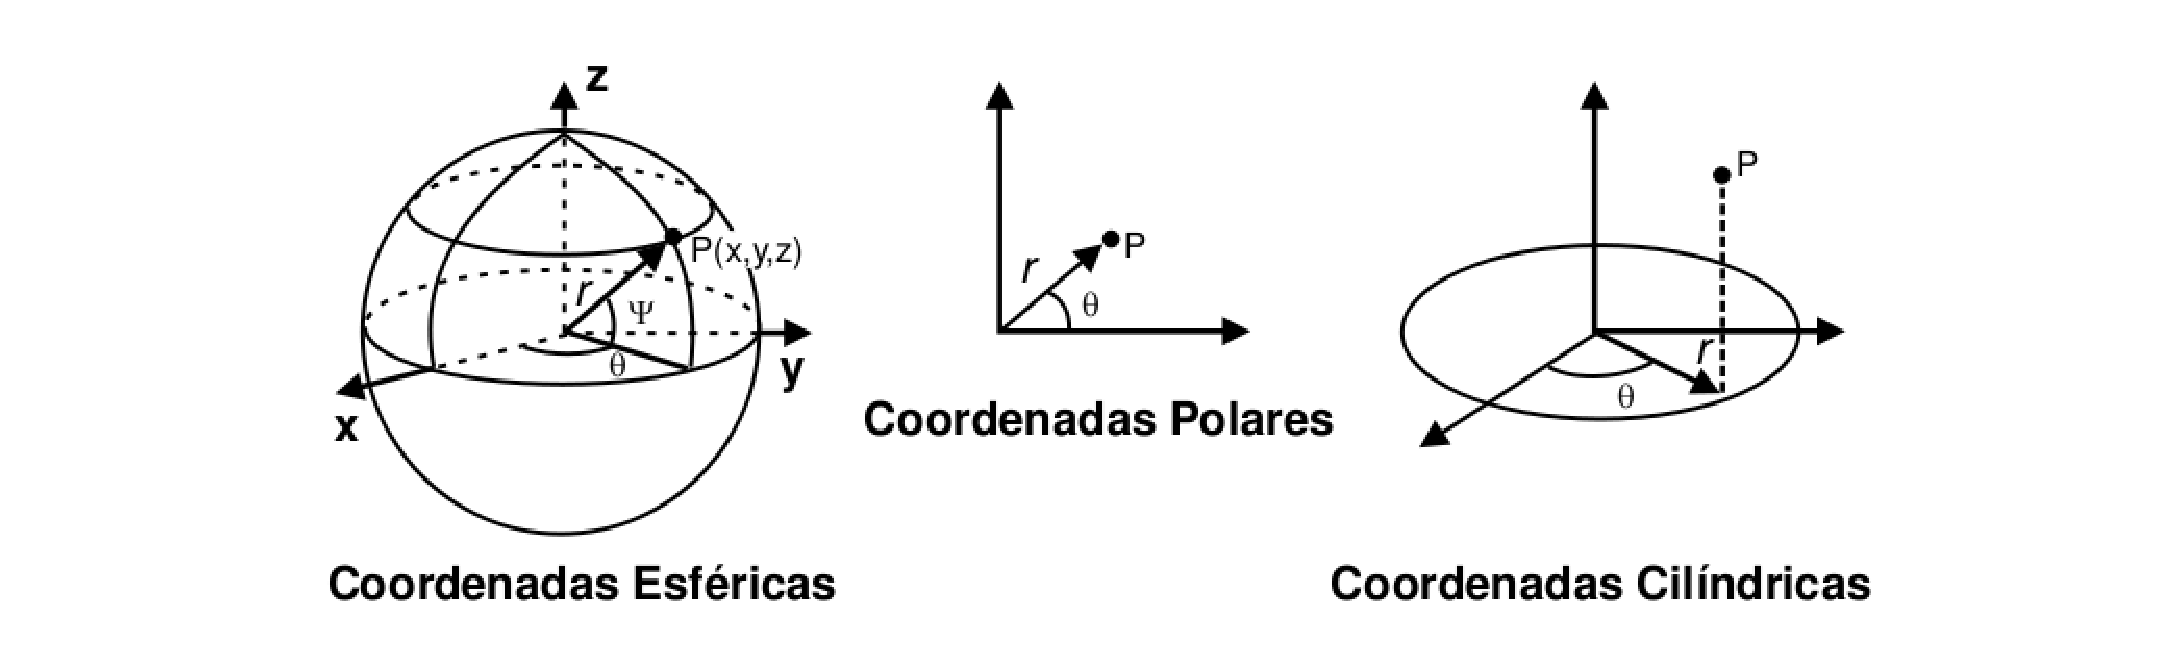
\includegraphics[scale=0.4]{s_coordenadas}
	\caption{Sistemas de coordenadas.}
	\label{fg:coordenadas}
\end{figure}

\subsection{Transformações}
As transformações são umas das características mais importantes da computação gráfica. Elas representam um mapeamento de ponto(s) de uma determinada posição para outra~\cite{comp_grafica1}. As transformações mais usadas e conhecidas são: rotação, escala e translação.\\

%--------------tranlasao---------------
Transladar significa mover o objeto. Essa operação é dada pela equação~\ref{eq:translacao}, onde adicionando quantias($T_x$, $T_y$ e $T_z$) a sua coordenada atual($x$, $y$ e $z$), obtém-se uma nova posição, transladada($x'$, $y'$ e $z'$). A Figura~\ref{fg:trans} mostra essa transformação. \\

\begin{equation}\label{eq:translacao}
[x'\ y'\ z'] = [x\ y\ z] + [T_{x}\ T_{y}\ T_{z}]
\end{equation}

\begin{figure}[ht!]
      \centering
	  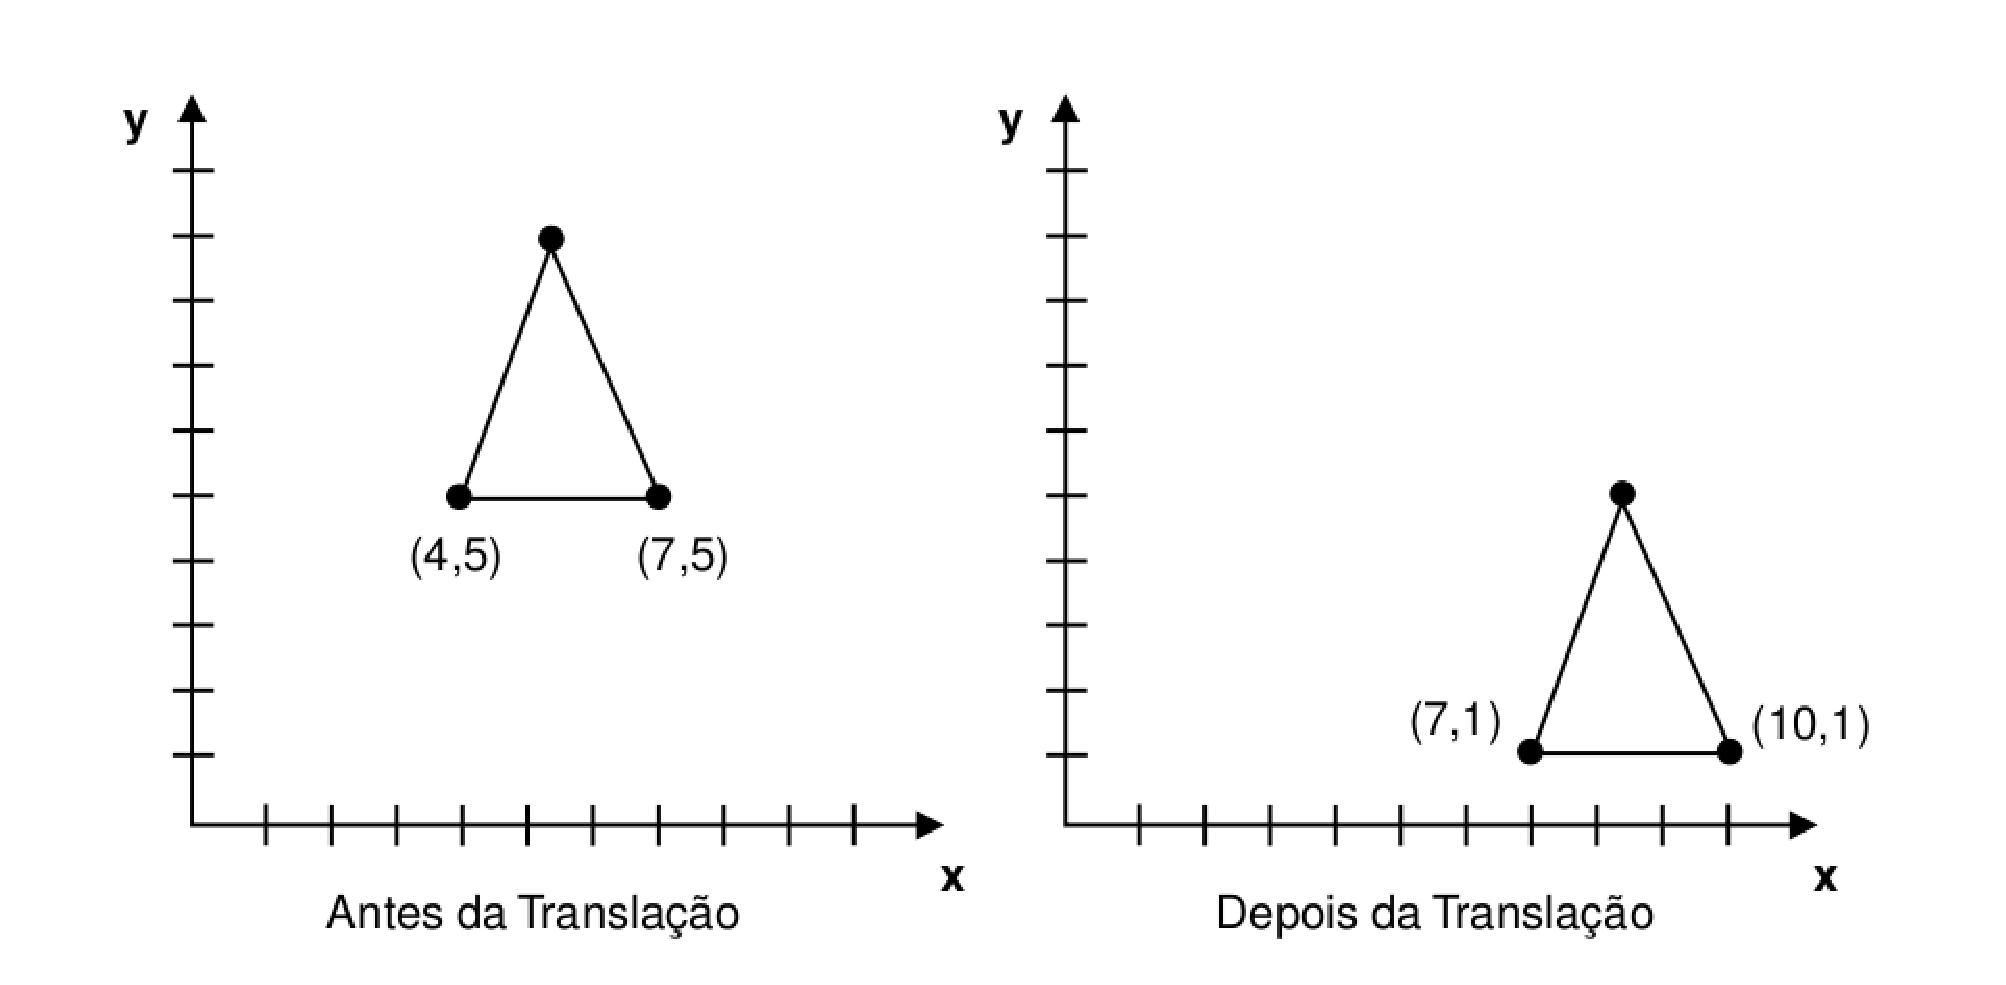
\includegraphics[scale=0.4]{trans}
	  \caption{Operação de Translação 2D.}
	  \label{fg:trans}
\end{figure} 

%--------------escala---------------
A operação de escala é aquela associada à mudança de dimensão dos objetos. Ela é representada pela equação matricial~\ref{eq:escala}, que mostra que quando multiplicamos as dimensões atuais ($x$, $y$ e $z$) por alguns fatores ($S_x$, $S_y$ e $S_z$), obtemos um novo objeto escalado ($x'$, $y'$ e $z'$). A Figura~\ref{fg:escala} mostra bem o que ocorre quando escalonamos um objeto.\\

\begin{equation}\label{eq:escala}
    \begin{array}{c c c}
    [x' \ y' \ z'] = [x \ y \ z]
    \begin{bmatrix}
     S_x & 0 & 0   \\[0.2em]
     0 & S_y & 0   \\[0.2em]
     0 & 0 & S_z
    \end{bmatrix}
    \
    = [xS_x\ yS_y\ zS_z]
    \end{array}
\end{equation}

\begin{figure}[ht!]
      \centering
	  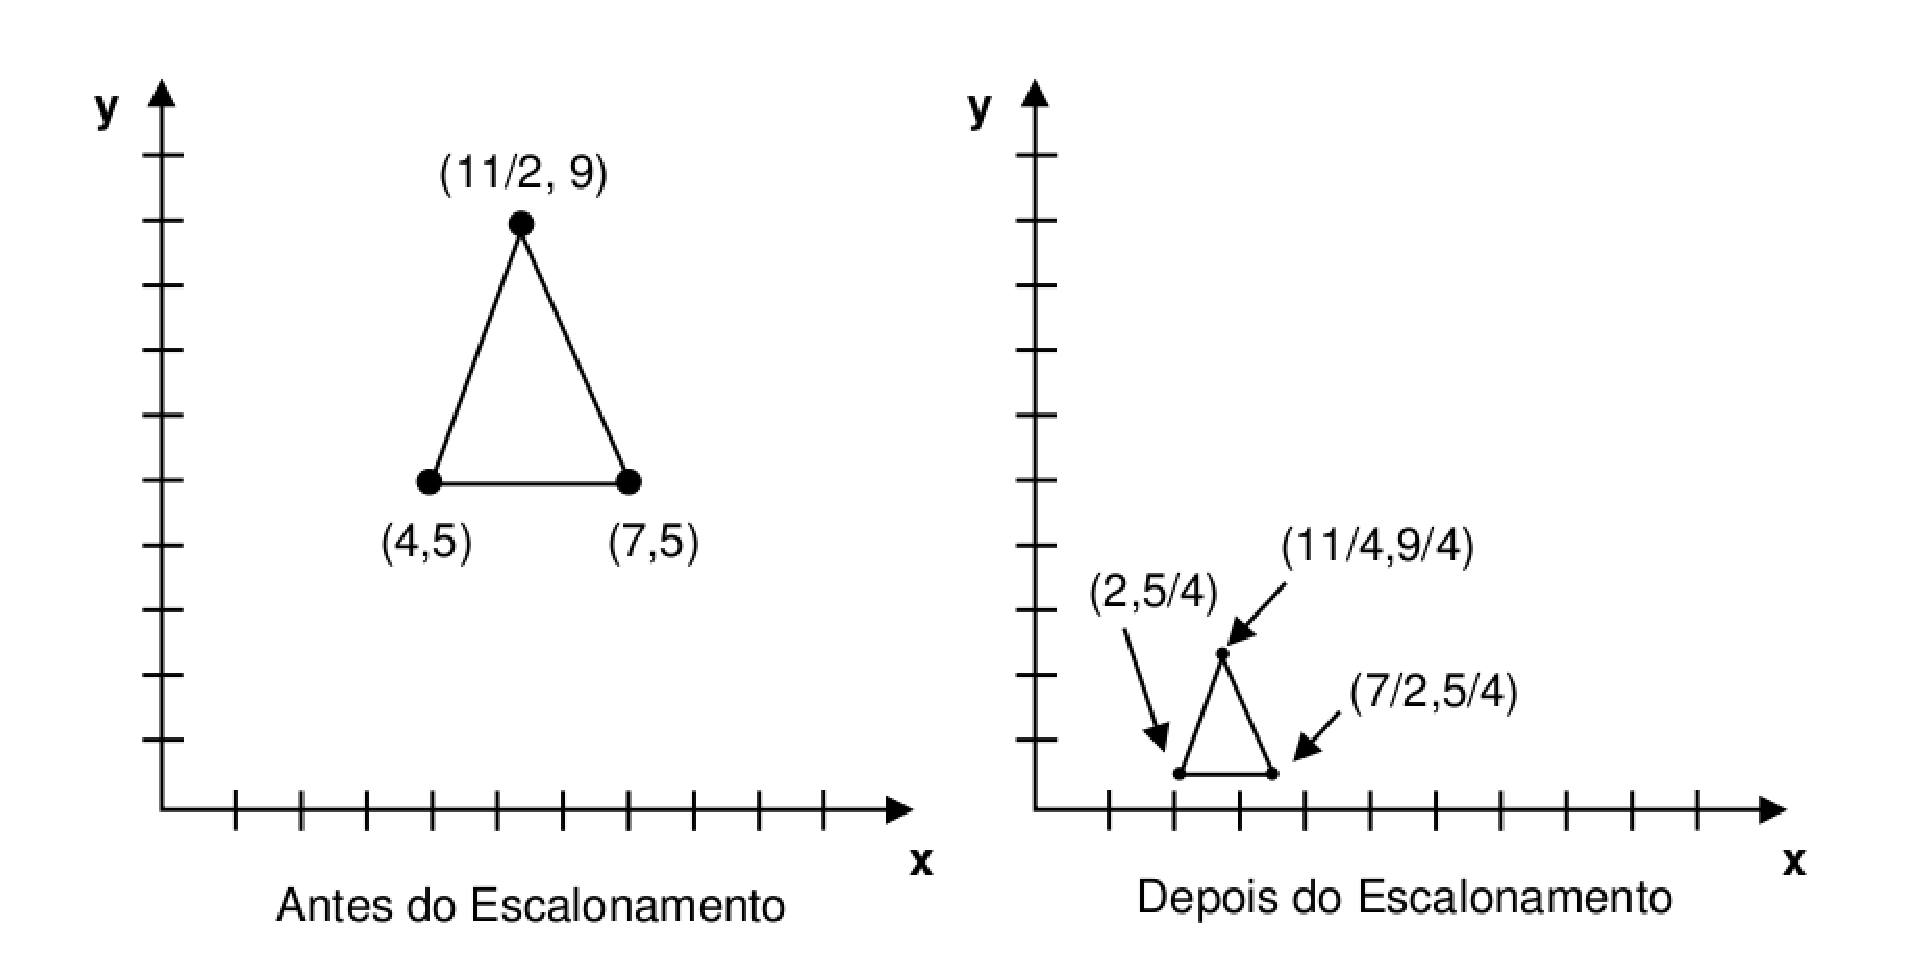
\includegraphics[scale=0.4]{escala}
	  \caption{Operação de Escala 2D.}
	  \label{fg:escala}
\end{figure} 

%--------------rotacao---------------
Por fim, quando desejamos girar um objeto ou um ponto no nosso sistema de coordenadas, usamos a transformação de rotação, a qual pode ser representada pelas formas matriciais~\ref{eq:rotacao}, que mostram, respectivamente, as matrizes rotação para os eixos $x$, $y$ e $z$. A Figura~\ref{fg:rotacao}, ilustra essa operação.

\begin{figure}[ht!]
      \centering
	  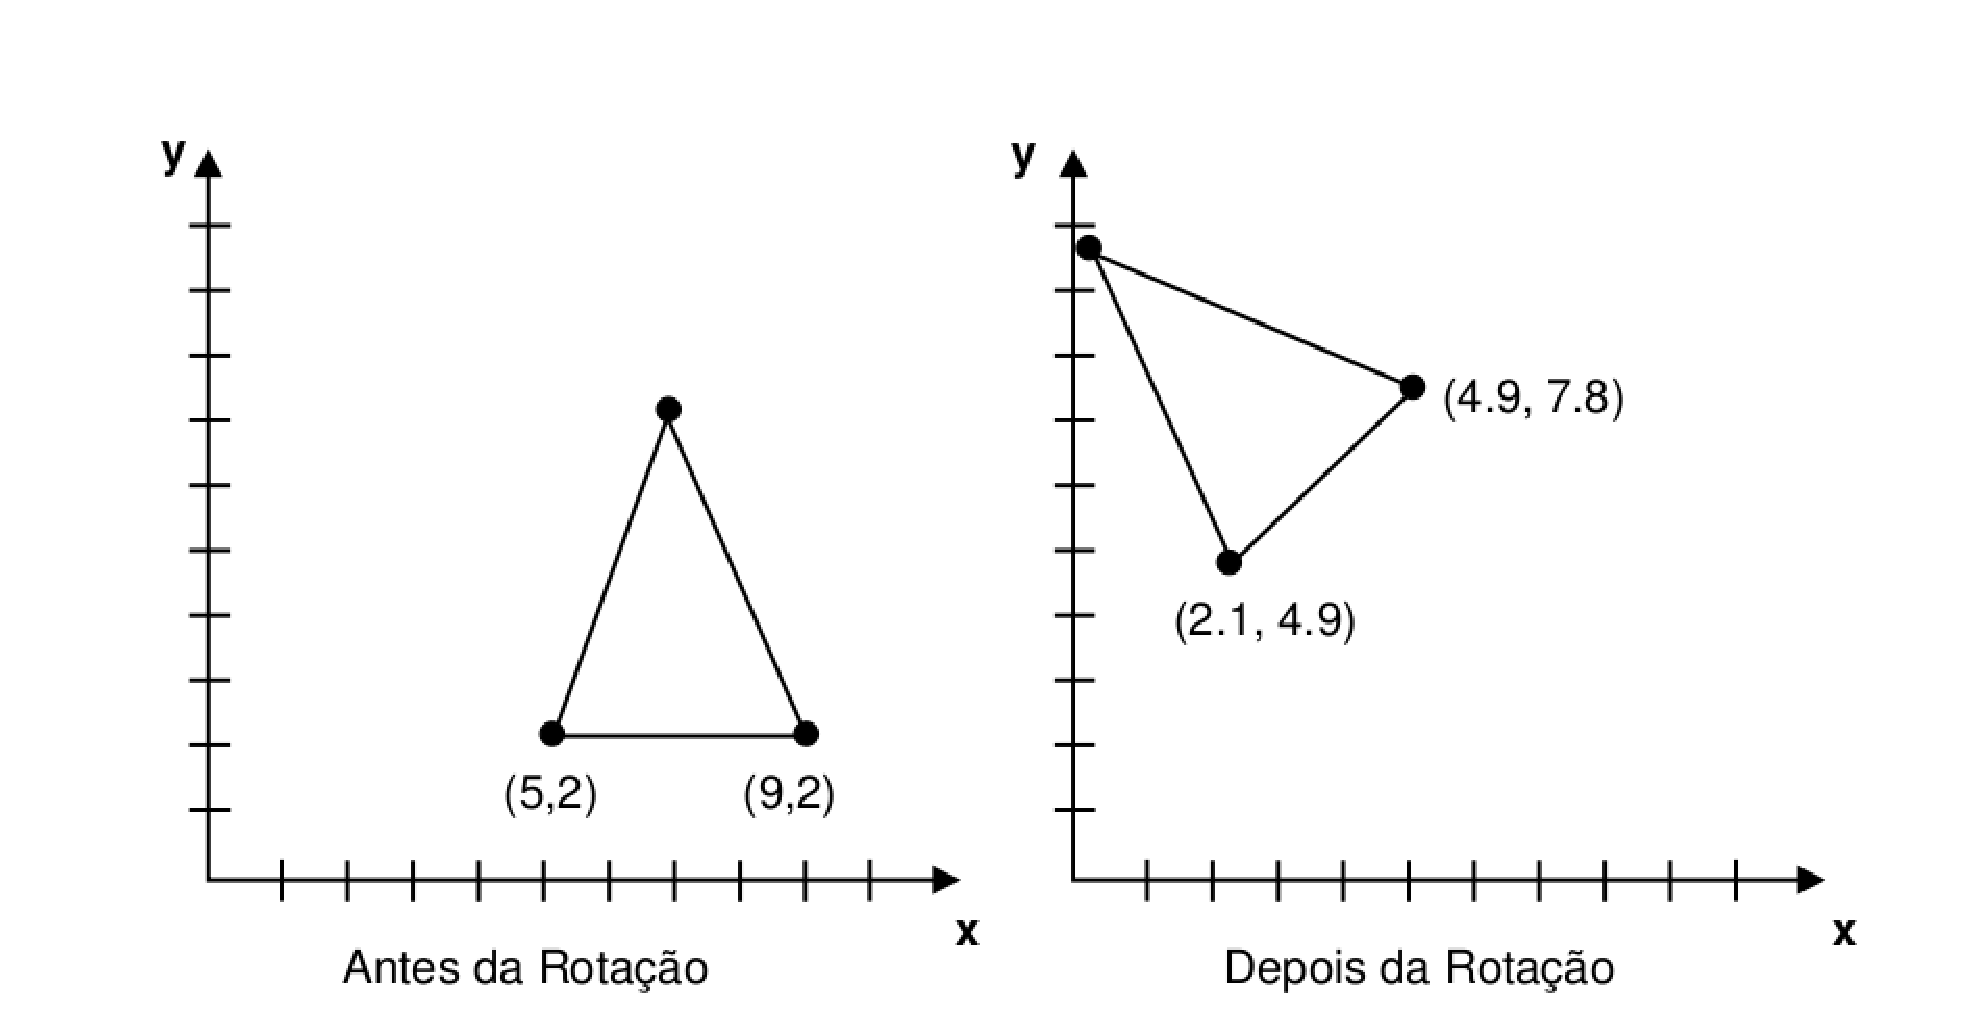
\includegraphics[scale=0.4]{rotacao}
	  \caption{Operação de Rotação 2D.}
	  \label{fg:rotacao}
\end{figure} 
\begin{center}
\begin{equation}\label{eq:rotacao}
  \begin{array}{c c c}
     R_x(\theta) = \begin{bmatrix}
    1 & 0 & 0   \\[0.2em]
    0 & \cos(\theta) & -\sin(\theta)    \\[0.2em]
    0 & \sin(\theta) & \cos(\theta) \\
    \end{bmatrix}
    , 
    R_y(\theta) = \begin{bmatrix}
    \cos(\theta) & 0 & \sin(\theta) \\[0.2em]
    0 & 1 & 0   \\[0.2em]
    -\sin(\theta) & 0 & \cos(\theta)\\
    \end{bmatrix}
    ,
    R_z(\theta) = \begin{bmatrix}
    \cos(\theta) & -\sin(\theta) & 0\\[0.2em]
    \sin(\theta) & \cos(\theta) & 0\\[0.2em]
    0 & 0 & 1\\\ 
    \end{bmatrix}
    \end{array}
\end{equation}
\end{center}

\subsection{Representação de Sólidos}
\subsubsection{Representação Armada ou Wireframe}
É a representação dada por um conjunto de arrestas que define as bordas do objeto\cite{speck}. Tem a vantagem de ser mais rápida quanto a renderização, porém tem um problema relacionado ao fato de dar margem para várias interpretações, além de dificultar cálculos como: volume e massa de sólidos. Por isso, ela geralmente não é considerada uma técnica de modelagem de sólidos. A Figura~\ref{fg:wireframe} esta ilustrando essa técnica.

\begin{figure}[ht!]
	\centering
	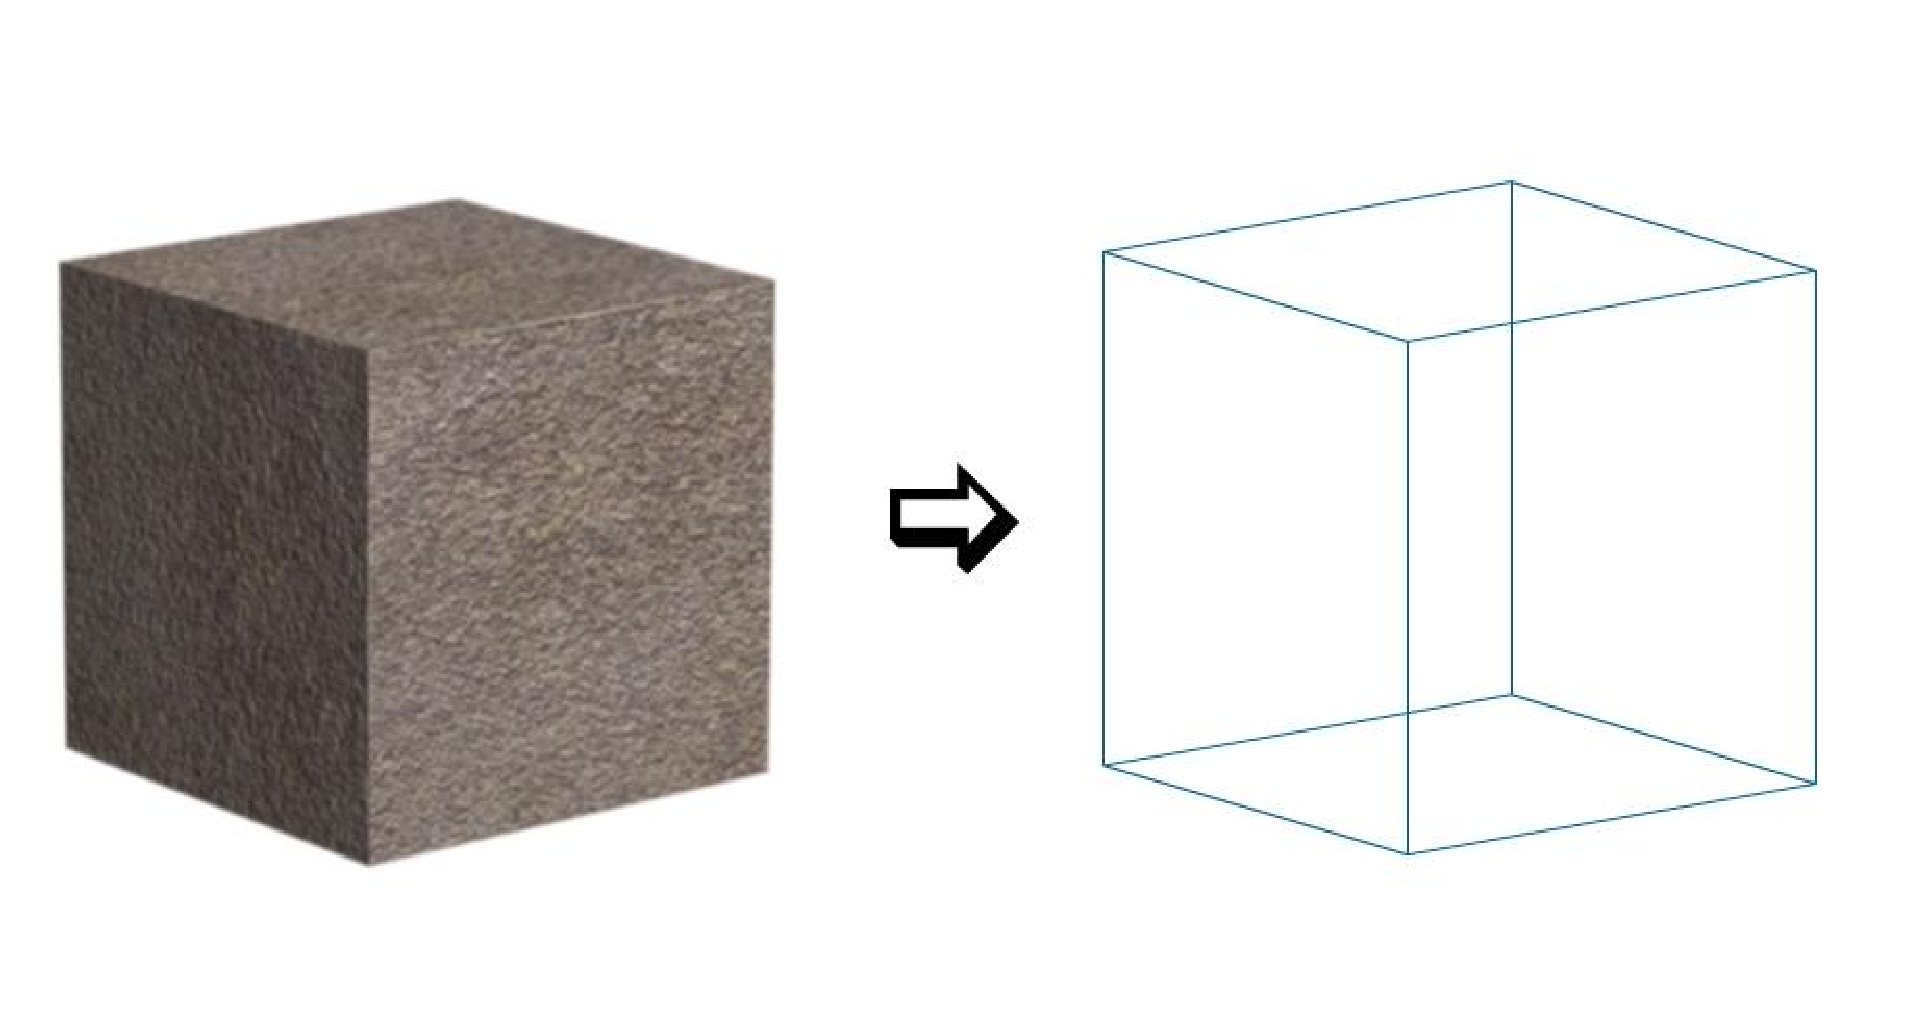
\includegraphics[scale=0.2]{wireframe}
	\caption{Representação Armada ou Wireframe.}
	\label{fg:wireframe}
\end{figure} 

\subsubsection{Representação por Faces} 
\label{sec:r_faces}
Usa faces delimitantes que descrevem os contornos do sólido. É uma das formas mais usuais na modelagem de objetos tridimensionais nos dias de hoje. Ela  também é conhecida com  \textbf{Boundary Representation} ou \textbf{B-rep}, que consiste na descrição de  objetos pelos seus contornos, ou seja, arestas e vértices. Para melhor entendimento, temos a Figura~\ref{fg:faces} como exemplo dessa representação.

\begin{figure}[ht!]
      \centering
	  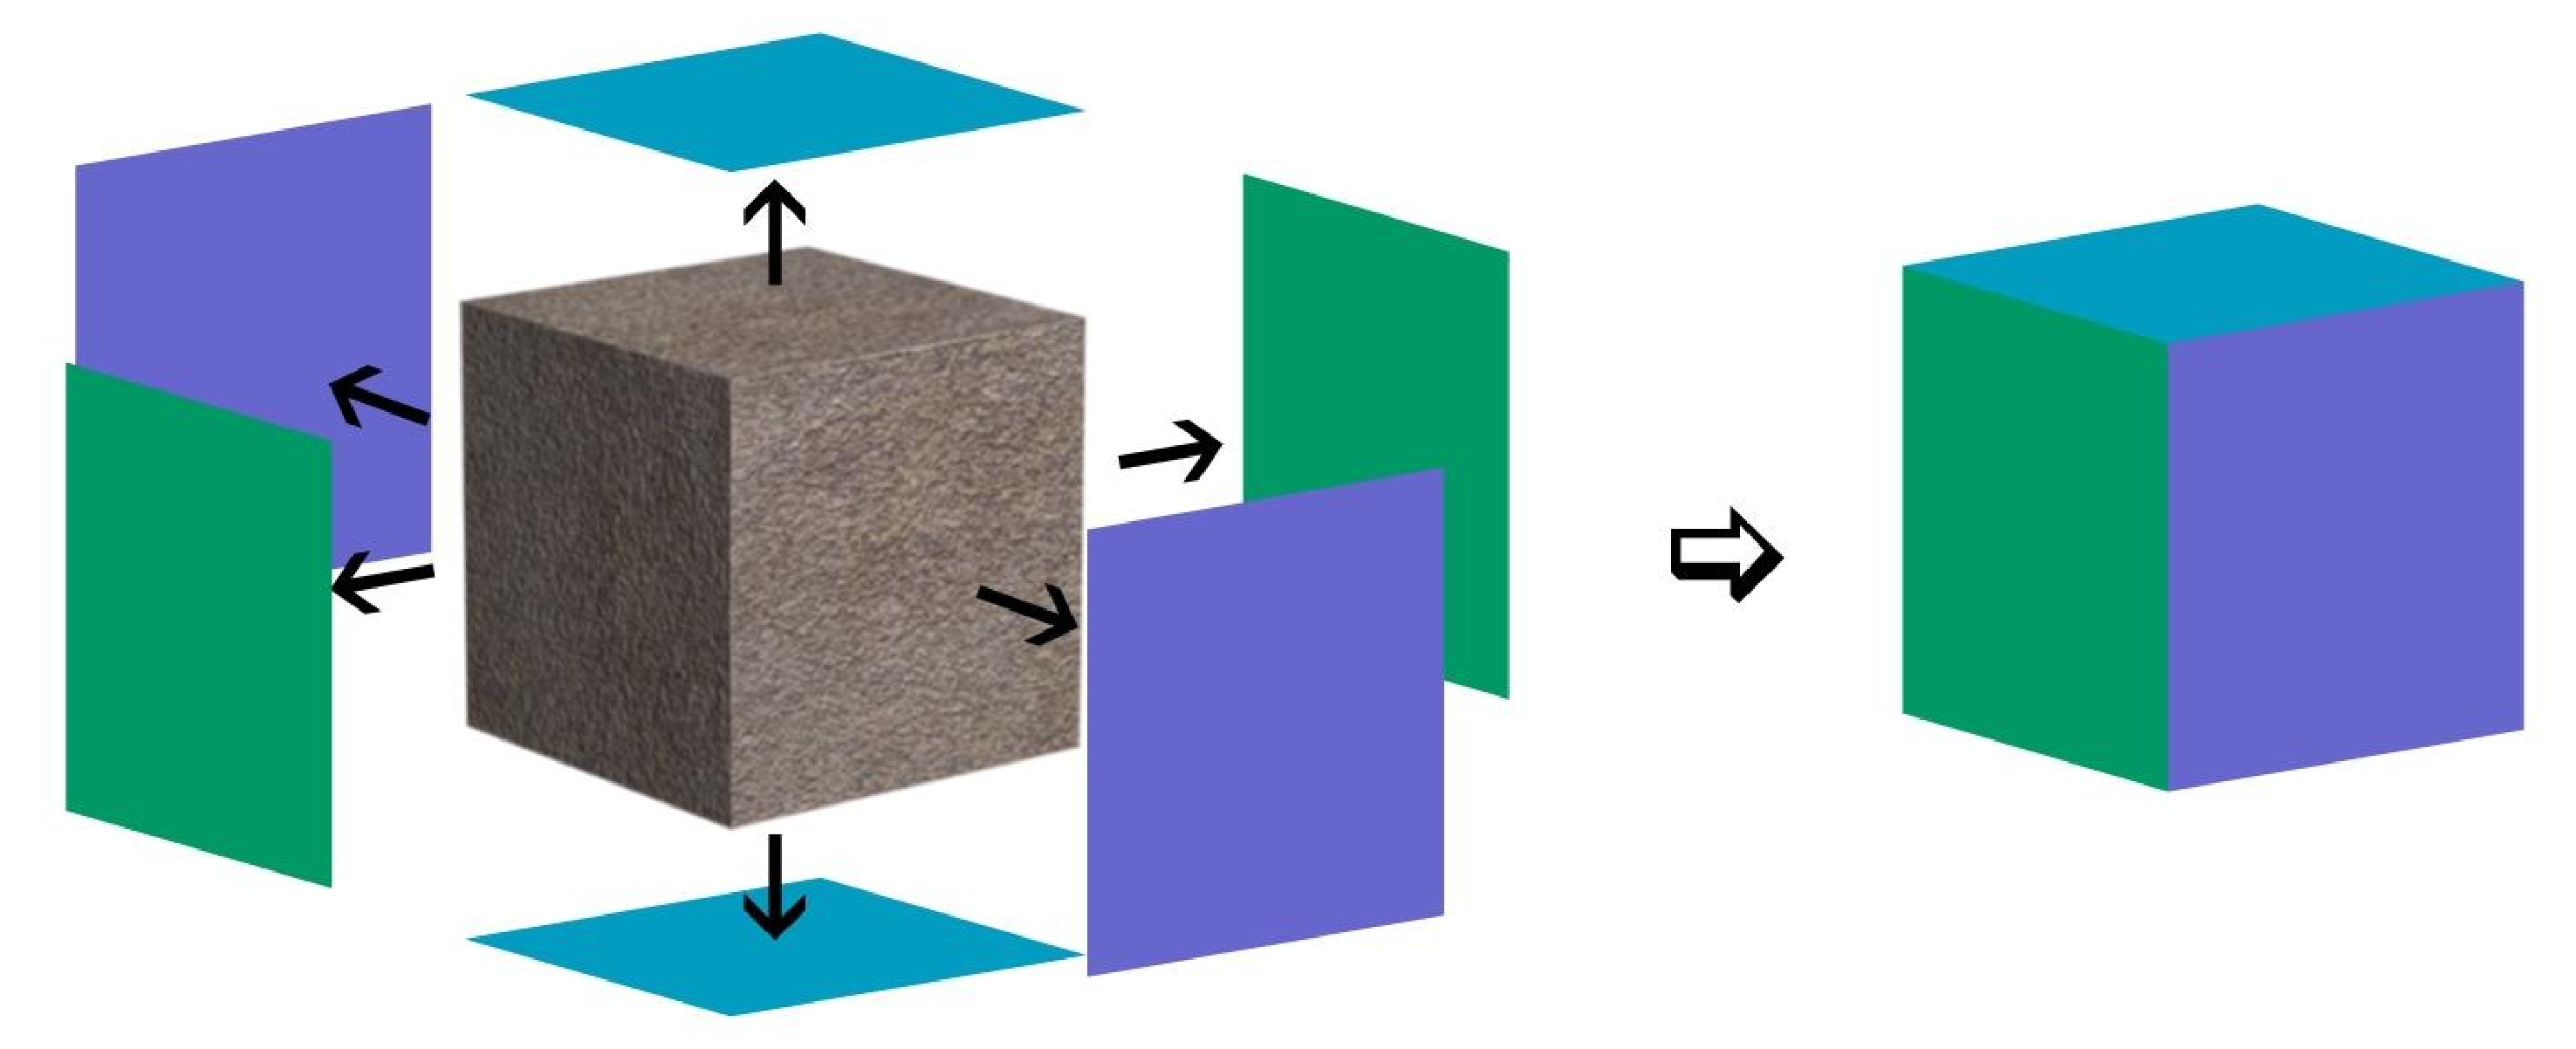
\includegraphics[scale=0.2]{faces}
	  \caption{Representação por Faces.}
	  \label{fg:faces}
\end{figure} 

\subsubsection{Representação Poligonal}
Polígono vem do grego \textit{polys}, que significa muitos , e \textit{gonos} que significa ângulos, assim esse representação é formada por figuras planas com muitos seguimentos de reta e muitos ângulos. Então podemos construir sólidos com o polígono mais  simples, o triângulo, até um mais complexo, com um número elevado de lados(Figura~\ref{fg:pilogono}). Essa técnica pode ser considerada uma especificação do caso apresentado na seção~\ref{sec:r_faces}.\\

\textit{Tesselation} é um das características dessa representação, significa preencher uma dada região através de várias repetições de um mesmo polígono até não haver mais espaços em "branco". A maioria das máquinas de jogos utilizam a representação por faces triangulares. Isso se deve ao fato de esta necessitar de menos processamento e também por possibilitar a representação de qualquer tipo de contorno\cite{traina}.

\begin{figure}[ht!]
      \centering
	  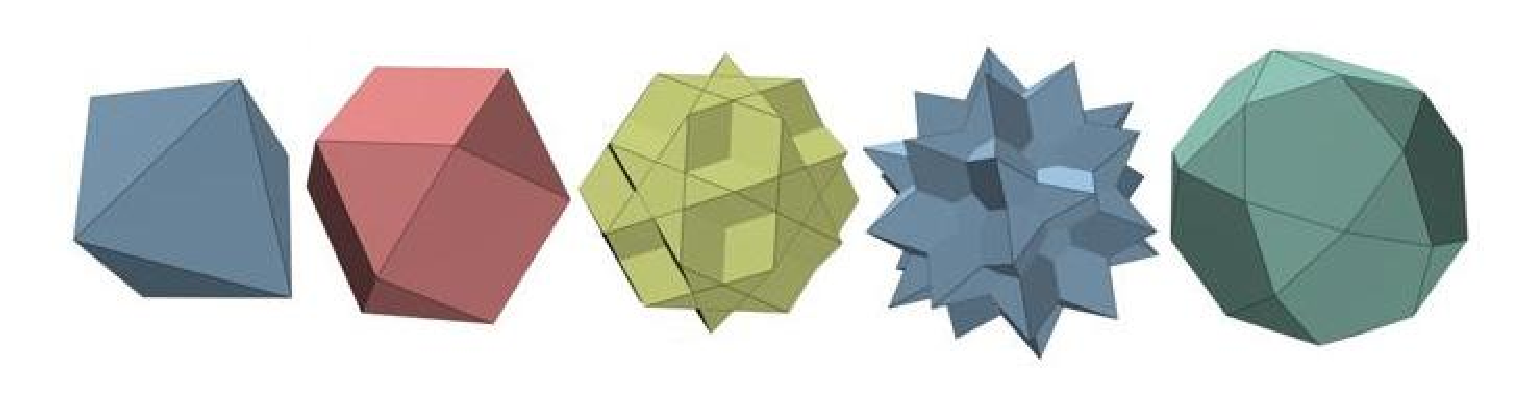
\includegraphics[scale=0.2]{poligonos}
	  \caption{Representação Poligonal.}
	  \label{fg:pilogono}
\end{figure} 

\subsection{Técnicas de Modelagem Geométrica}
Quanto ao âmbito da modelagem de objetos tridimensionais, tem-se basicamente três categorias: a manual, matemática e automática. \\

O método manual foi a base de toda a modelagem atual. É a técnica mais barata e mais antiga.  Utiliza-se basicamente das medidas do modelo real e, é claro, da habilidade do modelador. Já à matemática utiliza de algoritmos para gerar o objeto desejado. Esse método é muito utilizado para modelar, por exemplo, a proliferação de organismos microscópicos.\\

Modelagem automática é o método mais recente. Utiliza-se de scanners muitos sofisticados para obter o modelo tridimensional de qualquer ambiente ou sólido.

\subsubsection{Combinação de Objetos}
É um dos métodos mais intuitivos e antigos. É realizado através da combinação de um ou mais sólidos básico para obtenção de um outro\cite{hearn}, mostrado na Figura~\ref{fg:comb}. O  único detalhe que deve-se prestar bastante atenção nessa técnica, é a questão das operações booleanas(interseção, união e subtração) em alguns casos não gerarem como resultado um sólido, por exemplo, no caso da intercessão de dois cubos que não estão em contato, temos como resultado o vazio que não é um sólido válido.

\begin{figure}[ht!]
	\centering
	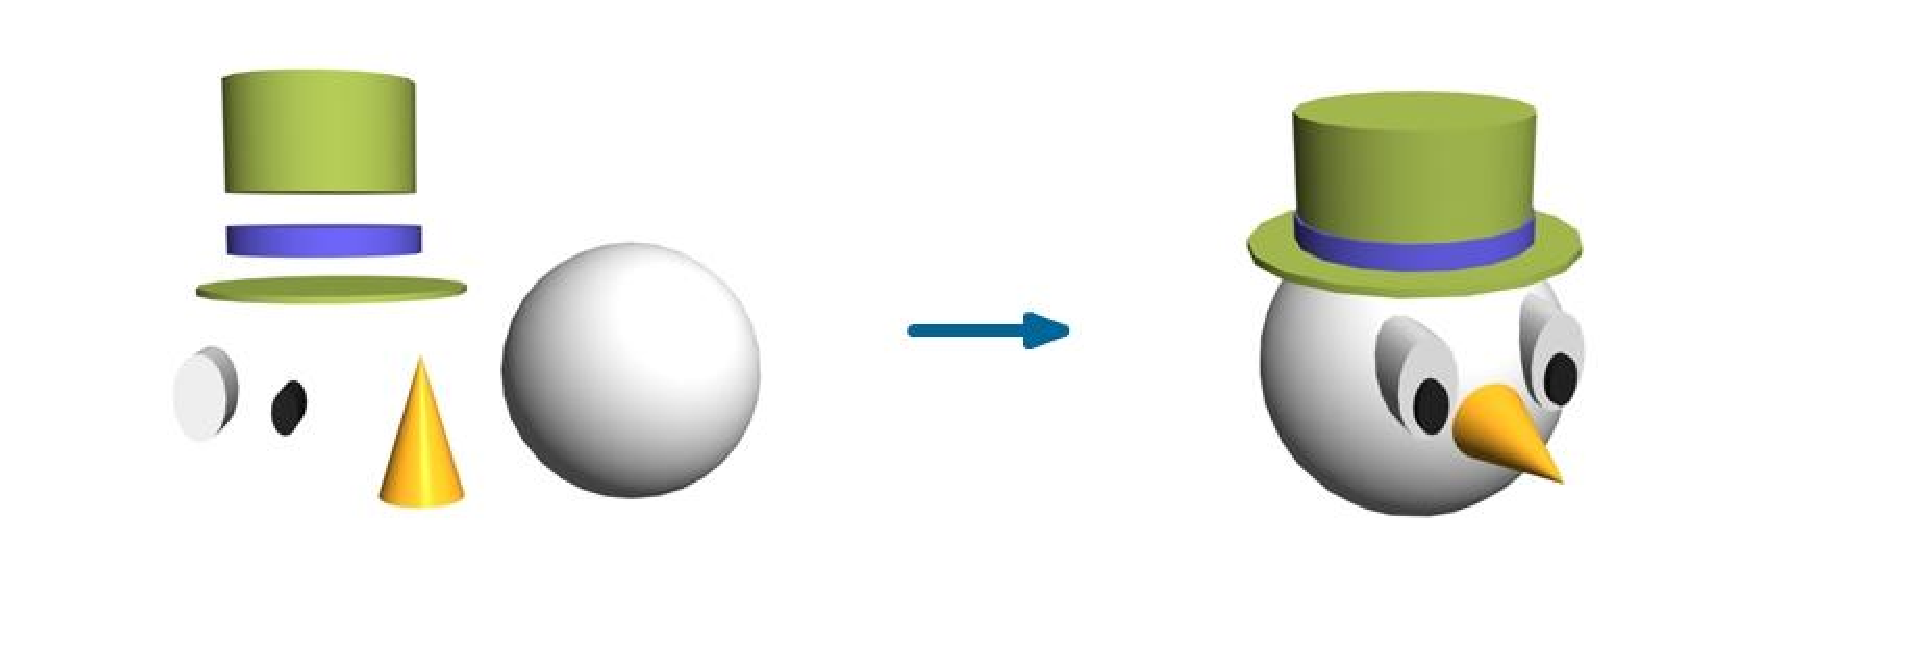
\includegraphics[scale=0.4]{montagem}
	\caption{Modelagem por Combinação de Objetos.}
	\label{fg:comb}
\end{figure} 

\subsubsection{Modelagem por Varredura(Sweep)}
A modelagem por varredura é obtida pela movimentação de uma curva $N_1$ na trajetória de uma outra curva $N_2$ que descreverá um superfície que poderá ser usada como sólido. Sendo $N_1$ nomeada de \textit{Curva de Contorno} e $N_2$ de \textit{Caminho ou Diretriz}\cite{3dsmod}.\\

Ainda no questão da varredura, pode-se sitar dois casos particulares que são: varredura por \textit{Extrusão}(Figura~\ref{fg:etrusao}) ou \textit{Translacional}(Figura~\ref{fg:rotacional}) e a \textit{Rotacional}. Para o a primeira é a translação de uma superfície na forma circular, por exemplo , ao longo de uma direção, gerando um sólido(no caso um cilindro). No segundo caso ocorre a rotação de uma superfície ao longo de um eixo ou ponto de referência, resultando também em um sólido.

\begin{figure}[ht!]
	\centering
	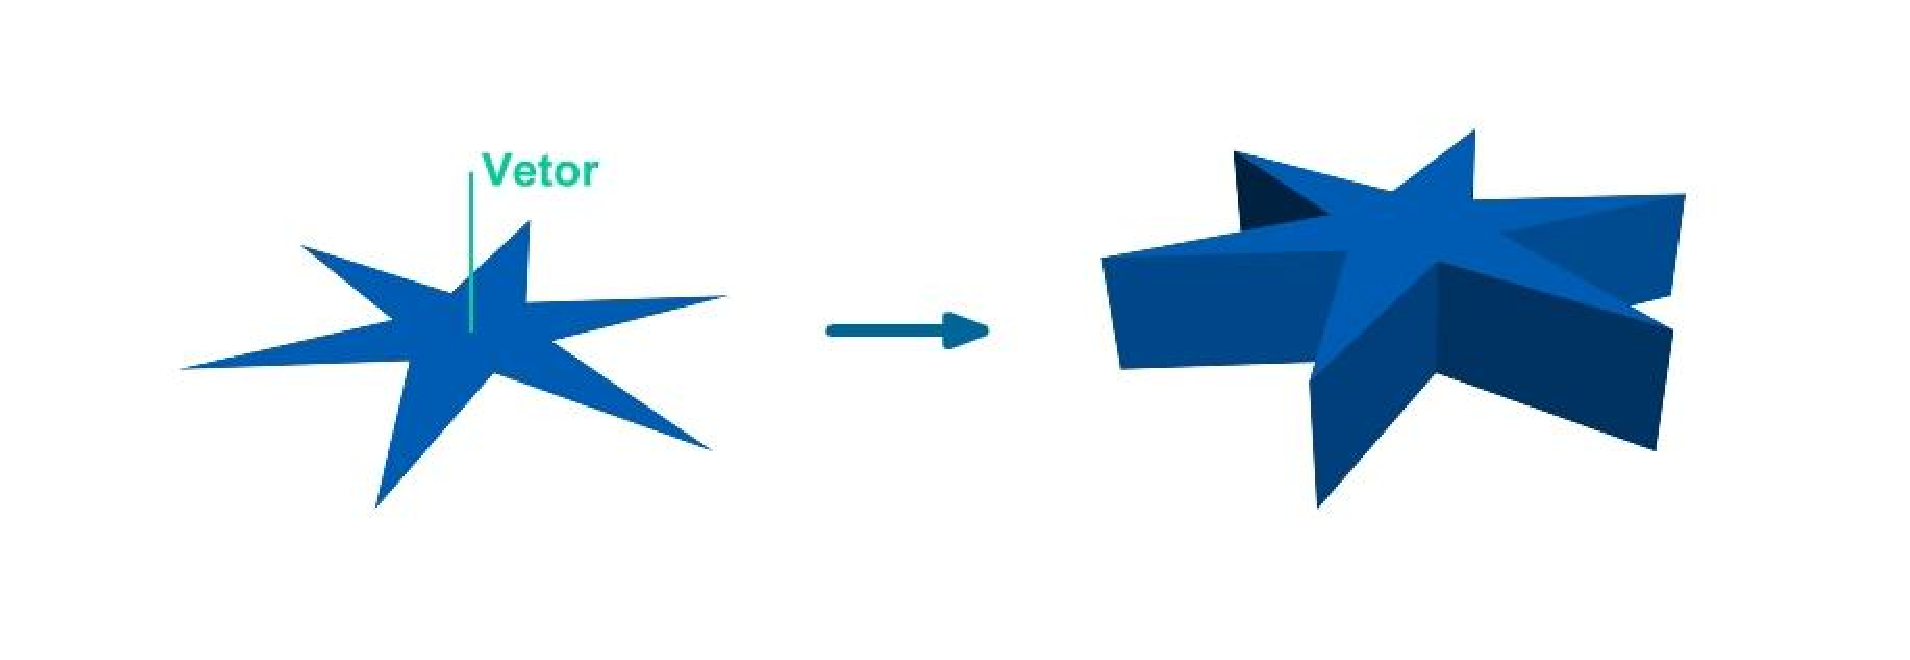
\includegraphics[scale=0.4]{extrude}
	\caption{Modelagem por Extrusão.}
	\label{fg:etrusao}
\end{figure} 
\begin{figure}[ht!]
	\centering
	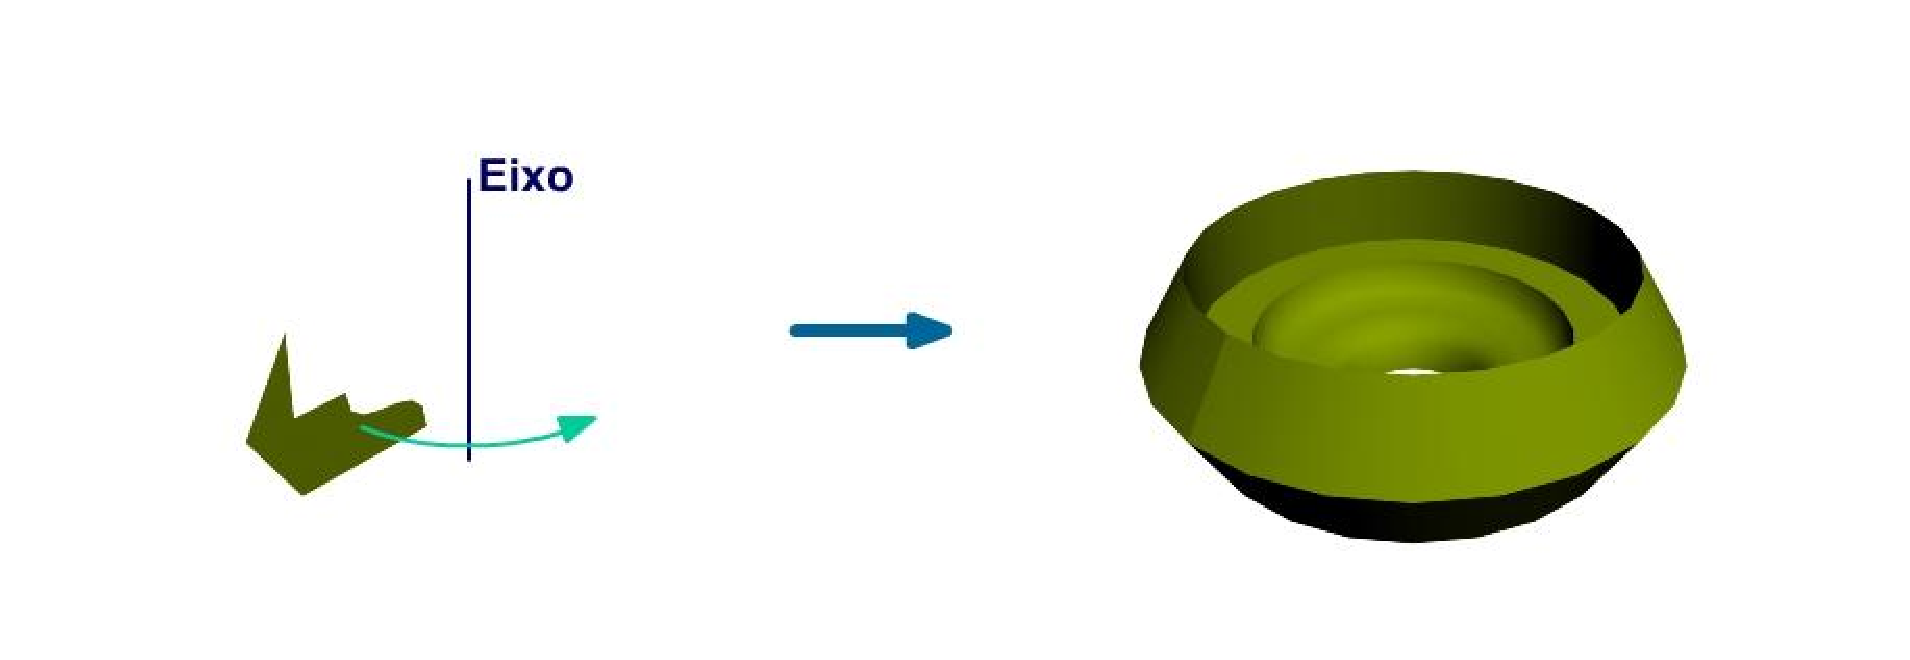
\includegraphics[scale=0.4]{rotacional}
	\caption{Modelagem Rotacional.}
	\label{fg:rotacional}
\end{figure} 

\subsection{Realidade Virtual}
O termo Realidade Virtual surgiu na década de 80 pelo artista e cientistas da computação, Jaron Lanier, que uniu os dois universos, que até então eram, muito distantes, o mundo real e o virtual\cite{jane}. Porém há registro de trabalhos anteriores a essa denominação, dentre eles esta o primeiro capacete que permitia imersão, e também pode-se falar do famoso SENSORAMA\cite{rhen}(que não obteve um grande sucesso comercial, pelo seu valor, mas com certeza foi um dos trabalhos que deram impulso para o futuro dos ambientes virtuais).\\

Mas o que é Realidade Virtual? É uma interface avançada que permite o usuário, navegar, modificar, interagir em tempo real com uma determinada aplicação. Existem basicamente dois tipos de realidade virtual quanto o fator imersão a imersiva e a não imersiva. A primeira é caraterizada por permitir ao usuário se sentir dentro do ambiente(através do uso de capacetes especiais, óculos, luvas, roupas, caves~\cite{cave}, sensores, entre outros dispositivos), já a segunda isso não ocorre(onde usa-se mouse, teclado, monitores , etc)\cite{aect}.

\subsubsection{Grafo de Cena}
É um dos conceitos mais importantes da teoria de jogos, e também da computação gráfica. Sua definição é a de ferramenta para representação de ambientes virtuais tridimensionais. Sendo esse ambiente descrito por diversos aspectos, dentre eles: descrição geométrica, câmera, transformação, aparência, comportamento e iluminação\cite{ferreira}. O cenário é formado por todos esses aspectos inseridos dentro do grafo de cena. \\

O grafo de cena é formado por nós, compondo arrestas que tem como resultado um grafo acíclico direcionado. Com cada nó tendo atributos ,sitados anteriormente, que poderão ou não influenciar nos outros nós que estão conectados a ele. Existe uma classificação para eles, que os divide em três categorias: nós raiz(é o primeiro nó, no qual todos os outros estão ligados de forma direta ou não) ,nós internos (geralmente contem informações de transformações 3D - rotação, escala e translação) e por fim estão os nós folha(que por padrão contem as dados de representação geométrica dos objetos da cena).\\ 

A propriedade fundamental dessa ferramenta é o que se chama de herança de estado. Que diz que cada nó deve herda as propriedades de estado do seus ancestrais até o nó raiz. Então se tivermos um grafo de cena formado por um \textit{nó} raiz, casa, e dois \textit{nós folha}, sendo o primeiro uma cadeira e o segundo mesa. Se rotacionarmos o \textit{nó} casa, por consequência teremos a cadeira e a mesa rotacionadas também. Porém no caso da rotação de um dos \textit{nós folha}, o \textit{nó} casa permanecerá inalterado, haja vista que ele esta hierarquicamente no nível acima e a cadeira também não se moverá pelo fato de ter uma ligação direta com esse nó(esta no mesmo nível e não tem conexão direta). Na tabela~\ref{tb:grafo_cena} estão algumas vantagens proporcionadas pelo uso dessa técnica.\\

\begin{table}
\centering
\begin{tabular}{|p{3cm}|p{8cm}|}
	\hline
	\multicolumn{2}{|c|}{Vantagens} \\ \hline
	Produtividade &  Gerencia e reduz o numero de linhas que seriam necessárias para implementar
a mesma funcionalidade utilizando uma interface de baixo nível, como a OpenGL.\\ \hline
	Portabilidade &  Encapsula todas as tarefas de baixo nível, reduzindo e até 
excluindo a parte de código que é especifica de uma plataforma.\\ \hline
	Escalabilidade &  Possibilita trabalhar tanto em máquinas com configurações básicas até supercomputadores.\\ 
	\hline
\end{tabular}
\caption{Vantagens proporcionadas pelo uso do grafo de cena.}
\label{tb:grafo_cena}
\end{table}

\section{Irrlicht}
O Irrlicht é uma máquina de jogo de alta performasse escrita em linguagem C++\cite{irrlichtbook}. Contem todas as característica que pode-se encontrar em qualquer outra \textit{engine}\footnote{Máquina de jogo.}. Existem muitos projetos desenvolvidos e em desenvolvimento usando-a, com uma boa comunidade, onde pode-se tirar dúvidas e publicar trabalhos e melhorias. E além de tudo isso, é completamente livre\cite{irrlicht}.\\

Ela tem como principais características:
\begin{enumerate}
\item Renderização em tempo real de alta performasse usando \textbf{Direct3D} e \textbf{OpenGL}.
\item Independe de plataforma.
\item Renderiza diretamente de arquivos, tais como : .zip, .pak, .pk3, etc.
\item Rápida e fácil detecção de colisão.
\item Possibilita o uso de vários linguagens de programação, como : Java, Delphi, entre outras.
\item Limpa, fácil de entender, e bem documentada.
\end{enumerate}

\section{Método FDTD}
O termo Método FDTD(Finite-Differene Time-Domain Method), primeiramente chamado de como Algorítimo de Yee, foi criado por Kane Yee em 1966\cite{yeebook}. É uma técnica capaz de solucionar, de forma simples e elegante, numericamente as equações de Maxwell, de maneira direta. Tem como características principais: 1)distribuição geométrica discreta das componentes de campos Elétrico e Magnético em células, de maneira a satisfazer tanto a Lei de Faraday quanto a Lei de Ampère nas formas diferencial e integral e 2)aproximação das derivadas espaciais e temporais por diferenças finitas, de forma a se obterem equações explicitas para a atualização temporal de todas as componentes de campo\cite{rodrigo}.\\

Porém, por algum tempo, esse método foi deixado de lado devido ao fato de ter um custo computacional muito alto, aliado a isso, deve-se levar em consideração o contexto histórico em que ele se encontrava, onde os computadores ainda eram bem limitados. Mas, um tempo depois, ressurgiu através dos trabalhos de dois cientistas, chamados Allen e Brodwin, que aplicaram essa técnica para problemas tridimensionais relacionados à interação eletromagnética com meios materiais\cite{allen}. Assim, novas técnicas apareceram e melhoram a abordagem do método, acompanhado , é claro, da evolução dos computadores.\\

Essa técnica tem sido usada desde então, em uma grande quantidade de aplicações, entre elas estão: radares, antenas, fotônica, sistemas de telecomunicação, medicina, estruturas periódicas, sistemas de aterramento, entre várias outras.\\

O método FDTD aplicado com intuito de simular uma propagação eletromagnética, utiliza as equações de Maxwell na forma diferencial.
\begin{equation}\label{eq:faraday}
	\overline{\nabla}\times\overline{E}=-\mu\frac{\partial \overline{H}}{\partial t},
\end{equation}
\begin{equation}\label{eq:ampere}
		\overline{\nabla}\times\overline{H}=\epsilon\frac{\partial \overline{E}}{\partial t} + \overline{J},
\end{equation}
		
	Onde:\\
	$\overline{J} = \sigma\overline{E}$, vetor densidade de corrente elétrica  de condução(ampere/$m^{2}$).\\ 

As equações (\ref{eq:faraday}) e (\ref{eq:ampere}) expandidas em coordenadas retangulares, geram as respectivas equações escalares, mostradas abaixo.
\begin{equation}
	\frac{\partial H_x}{\partial t} = \frac{1}{\mu}(\frac{\partial E_y}{\partial z}-\frac{\partial E_z}{\partial y}),
\end{equation}
\begin{equation}
	\frac{\partial H_y}{\partial t} = \frac{1}{\mu}(\frac{\partial E_z}{\partial x}-\frac{\partial E_x}{\partial z}),
\end{equation}
\begin{equation}
	\frac{\partial H_z}{\partial t} = \frac{1}{\mu}(\frac{\partial E_x}{\partial y}-\frac{\partial E_y}{\partial x}),
\end{equation}

\begin{equation}
	\frac{\partial E_x}{\partial t} = \frac{1}{\epsilon}(\frac{\partial H_z}{\partial y}-\frac{\partial H_y}{\partial z} -\sigma E_x),
\end{equation}
\begin{equation}
	\frac{\partial E_y}{\partial t} = \frac{1}{\epsilon}(\frac{\partial H_x}{\partial z}-\frac{\partial H_z}{\partial x} -\sigma E_y),
\end{equation}
\begin{equation}
	\frac{\partial E_z}{\partial t} = \frac{1}{\epsilon}(\frac{\partial H_y}{\partial x}-\frac{\partial H_x}{\partial y} -\sigma E_z)
\end{equation}

sendo:\\
$E_x, E_y, E_z$ e $H_x, H_y, H_z$ representam as componentes dos campos elétrico $\overline{E}$ e magnético $\overline{H}$, respectivamente. Essas componentes são funções do tempo $t$ e das três coordenadas cartesianas ($x,y,z$).\\

A lei de Faraday, equação (\ref{eq:faraday}), informa que quando há variação no tempo do vetor $\overline{B}=\mu\overline{H}$ (vetor densidade de fluxo magnético, em teslas), surgem componentes de campo elétrico circulando em torno da(s) componente(s) deste vetor. Já a lei de Ampère, equação (\ref{eq:ampere}), informa que quando há variação no tempo do vetor $\overline{D}=\epsilon\overline{E}$ (vetor densidade de fluxo elétrico, em ) em certa direção e/ou a presença da fonte de corrente $\overline{J}$, esta causa circulação de campo magnético em torno da direção da(s) componente(s) deste vetor.\\
			
Kane Yee se baseou nessa duas observações para definir seu esquema  de distribuição espacial  e temporal das componentes  de campo  de seu algoritmo. Sua representação geométrica, chamada de célula de Yee, esta mostrada na Figura \ref{fg:celulaYee}\cite{rodrigo}.\\
			
\begin{figure}[ht!]
\centering
	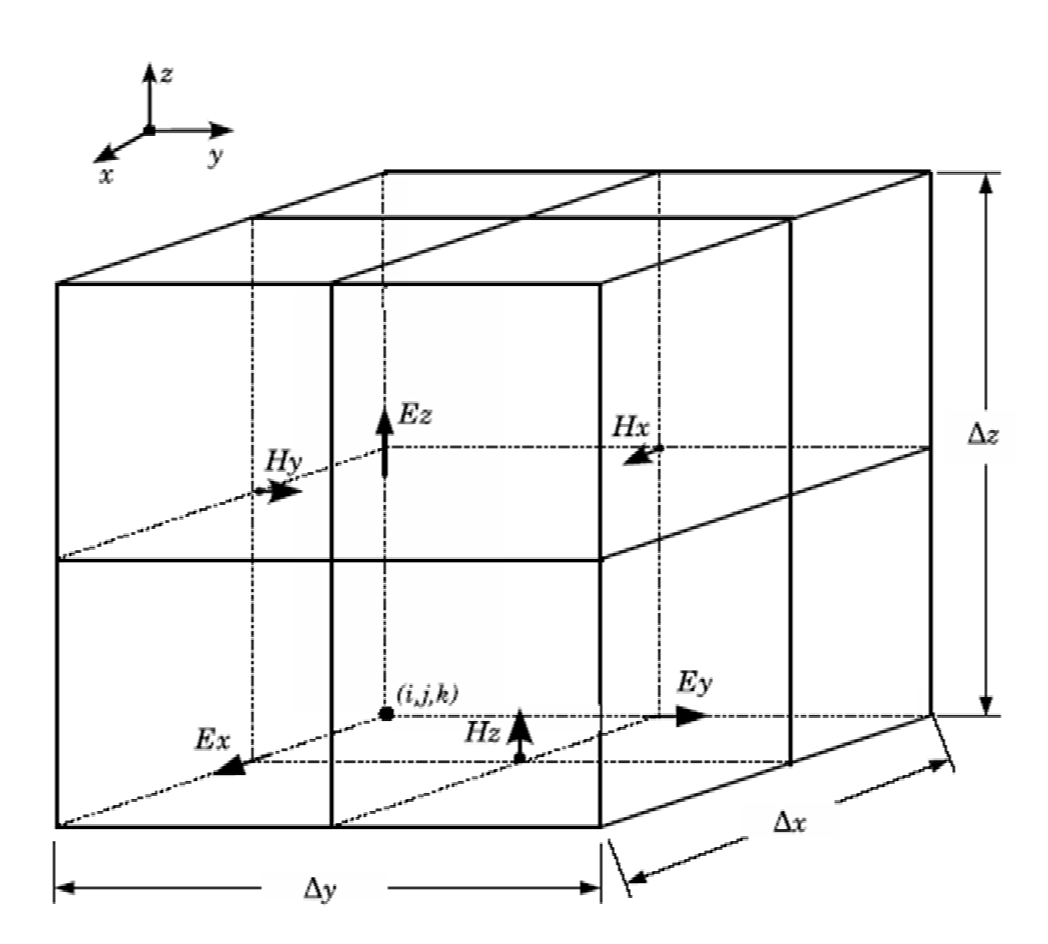
\includegraphics[scale=0.5]{celula}
	\caption{Célula Yee.}
	\label{fg:celulaYee}
\end{figure} 
		
Para que possam ser realizadas simulações de propagação de onda em FDTD, é criada uma malha 3D formada por múltiplas células de Yee que preenche toda região de análise, Figura\ref{fg:grade}\cite{almeida}, com a finalidade de mostrar as componentes de campo $\overline{E}$ e $\overline{H}$ atuantes em cada ponto da malha desta região.	\\
\begin{figure}[ht!]
	\centering
	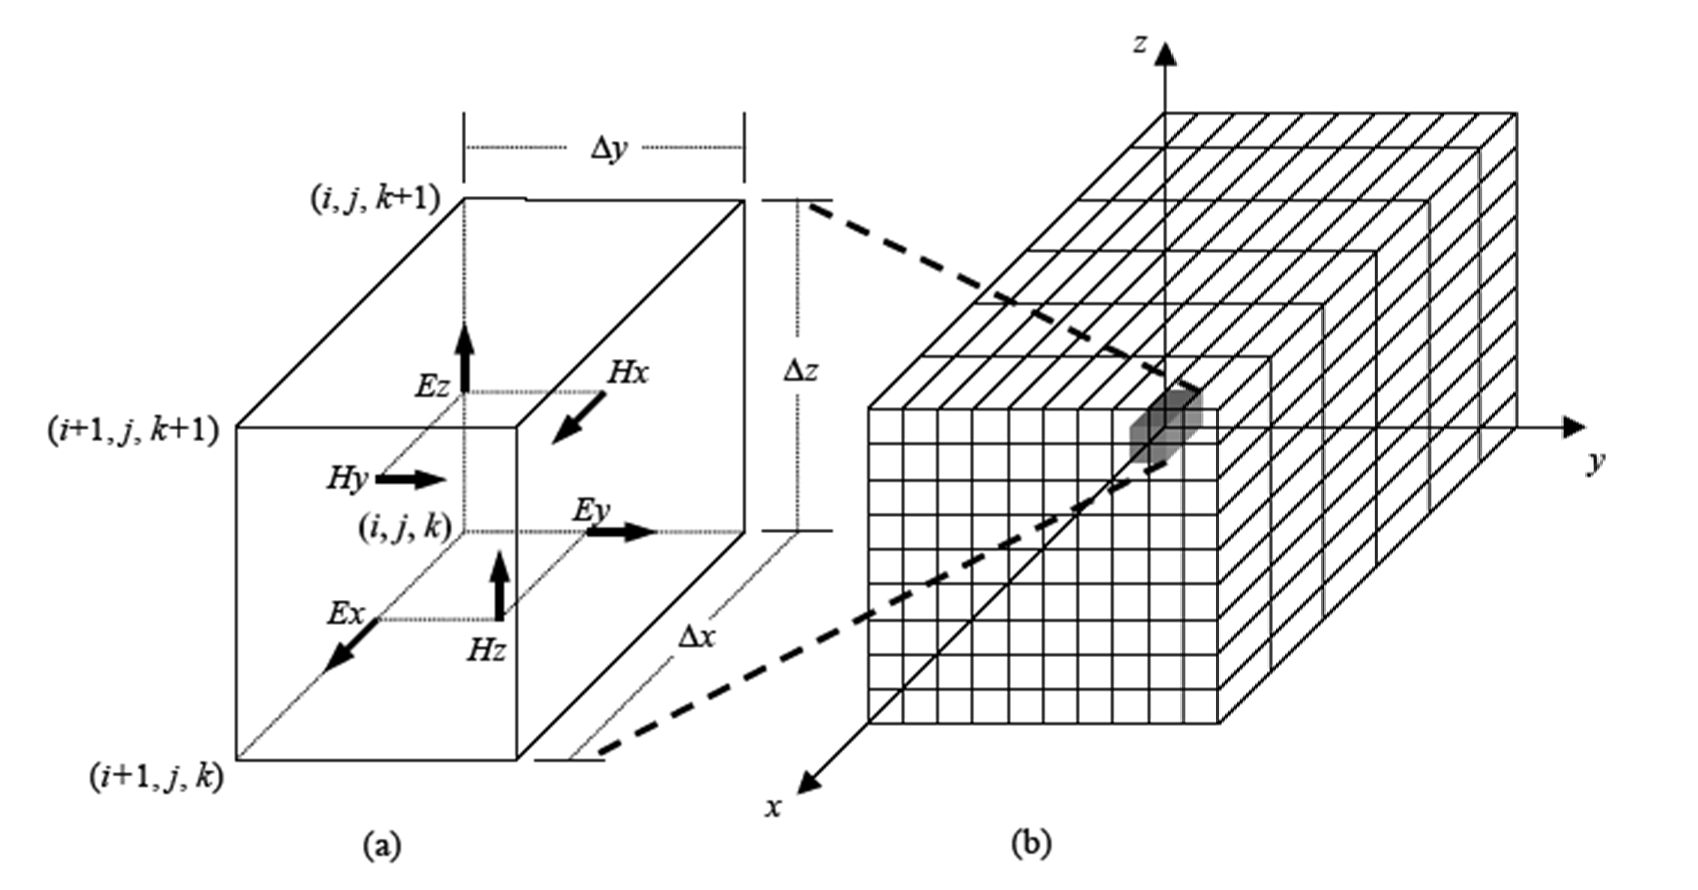
\includegraphics[scale=0.5]{Malha3D}
	\caption{(a) Posição das componentes dos campos elétrico e magnético em uma célula de Yee;(b) Célula no interior de uma malha 3-D.}
	\label{fg:grade}
	\end{figure} 

A referência a cada célula que compõe a malha, assim com as suas respectivas componentes de campo, é feita de forma discreta pelos índices $i, j$ e $k$, de forma que uma determinada posição $x, y, z$ (em metros) é referenciada no espaço discreto por $i, j, k$ (número da célula correspondente). Estas  referências são obtidas através das relações $x = i.\Delta_x, y = j.\Delta_{y}$ e $z = k.\Delta_z$, onde  $\Delta_x,  \Delta_y$ e $\Delta_z$ são as dimensões das células de Yee(Figura\ref{fg:celulaYee}).


\chapter{Desenvolvimento do Software}
%Como o avanço da computação foi e é grandioso, é normal e esperado que abranja área que antes ele não alcançava. Então, cada vez mais, o mercado, as pessoas, as empresas necessitam e requisitam softwares com finalidades variadas e assim fazendo com que surgirem vários ramos de desenvolvimento. Então surgiu a necessidade de criação de um padrão de desenvolvimento, para não somente auxiliar como também definir limites e regras para: criação, documentação e manutenção. Assim surgiu a engenharia de software.\\

%Para essa aplicação escolheu-se o modelo de desenvolvimento sequencial ou cascata(Figura~\ref{fg:modelo_dev}), que é uns dos mais antigos e também mais utilizados. 
%\begin{figure}[ht!]
%	\centering
%	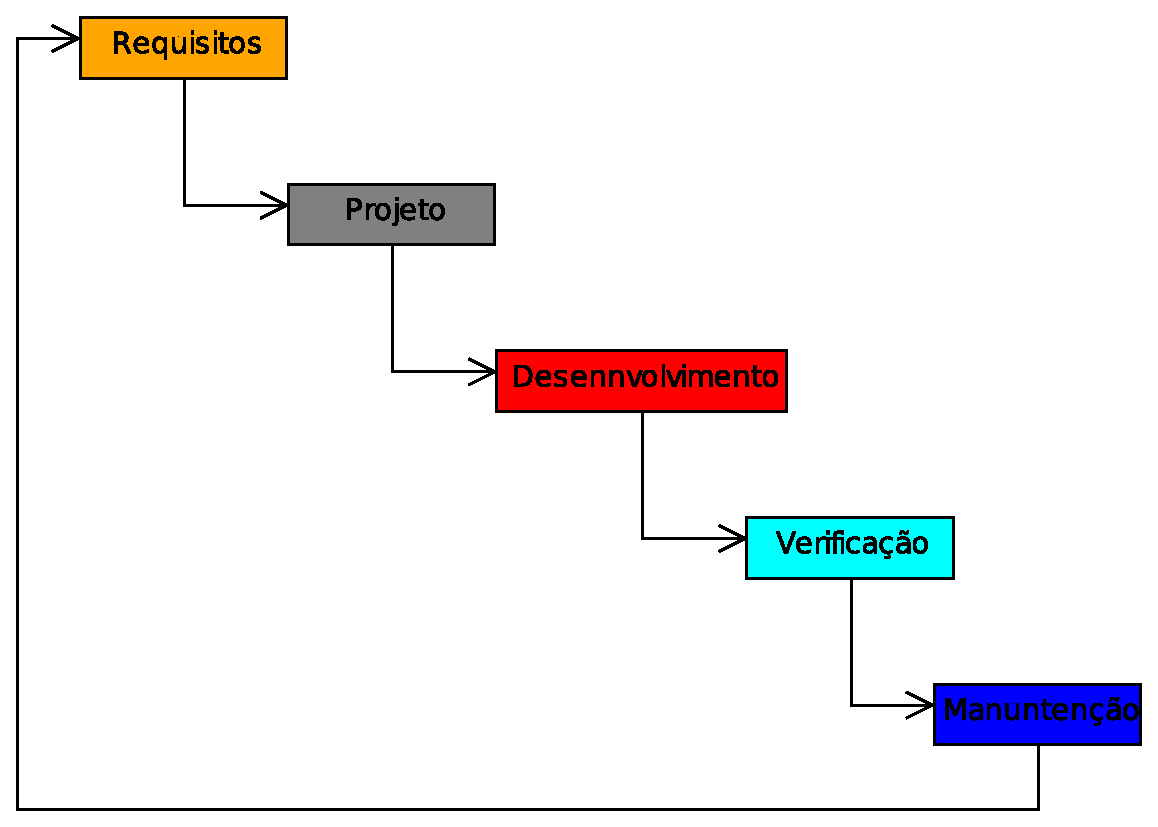
\includegraphics[scale=0.35]{modelo_dev}
%	\caption{Modelo de desenvolvimento cascata.}
%	\label{fg:modelo_dev}
%\end{figure}

	\subsection{Tecnologias de Programação Usadas} 
	As tecnologias de programação usadas foram: o motor gráfico de jogos irrlicht, a plataforma Qt-Creator e a linguagem C++. As informações sobre a engine irrlicht estão na seção $2.2$. O Qt-Creator é um poderoso ambiente multi plataforma que permite a criação de diversas aplicações web e também desktop. O uso dele, neste trabalho, foi voltado para a criação de uma interface desktop, a qual pudesse ser usada em diferentes sistemas operacionais(Linux, Windows ou Macintoch) e com arquiteturas dissemelhante(32 ou 64 bits). Tanto essa plataforma quanto a linguagem foram escolhidas por serem muito usadas pelo comunidade desenvolvedora, por serem robustas e terem uma ótima documentação.
	
	\subsection{Conexão Qt-Irrlicht}
	O primeiro passo no desenvolvimento desse trabalho foi a união do universo irrlicht com a plataforma Qt-Creator. Para tanto foi necessário o estudo das classes e funcionalidades básicas desse dois mundos.\\
	
	A ideia era colocar o motor gráfico irrlicht funcionando como uma janela dentro da interface gerenciada pelo qt. Assim criou-se a classe base de todo esse projeto, chamada IrrViewer. Ela contem os métodos base de uma classe Widget\footnote{Janela padrão do qt.}, que são : paintEvent(), resizeEvent() e paintEngine(); e também os necessários para a criação de um cenário 3D irrlicht, os quais são : createIrrlichtDevice()(reponsável pela criação do \textit{device}\footnote{Responsável por todas as informações da cena}, \textit{smgr}\footnote{Gerenciador de cena, ele que responsável por adicionar, remover, clonar e capturar objetos da cena.} e \textit{video-driver}\footnote{Responsável por tudo referente ao driver de video}), cenaIrrlicht()(método que tem a finalidade de criar a cena), drawIrrlichtScene()(método de pintura).\\
	
	Assim, com o Qt-Creator reconhecendo essa nova classe como uma janela(Widget) normal, pode-se passar para outra fase proposta, que era a criação de outras classes e métodos necessários para concretização do requisitos pré-estabelecidos para esse trabalho.

	\subsection{Classes}
	As classes criadas para este projeto foram: \textit{IrrViewer, Cena, IrrNode, ReceiverEvent} e \textit{MainWindow}. A primeira é a base de todo o desenvolvimento do software produzido nesse projeto, é a que conectar o irrlicht com o Qt. A classe \textit{Cena} contem e controla tudo referente a cena,tal como: seleção, inserção, modificação e deleção de \textit{nós}; Assim como também a geração de malha e eventos de mouse e teclado. A terceira classe é responsável pela criação de objetos: prisma, cubo, esfera, cone, haste, cilindro e antena.\\
	
	Já a classe \textit{ReceiverEvent} tem como finalidade receber os eventos de mouse do Qt e repassá-los para a engine irrlicht. Por fim, temos a classe MainWindow que é a interface em si, onde se encontram os botões e \textit{signals and slots}\cite{qt}.

\section{Interface}
A interface feita nesse projeto esta representada na Figura~\ref{fg:layout}. Ela foi baseada nos softwares de modelagem mais usados no mercado, que são : Blender, 3DStudio e Maya. A sua estrutura foi dividida em 4 áreas: barra superior, janela da cena, painéis laterais e barra inferior.\\

\begin{figure}[ht!]
	\centering
	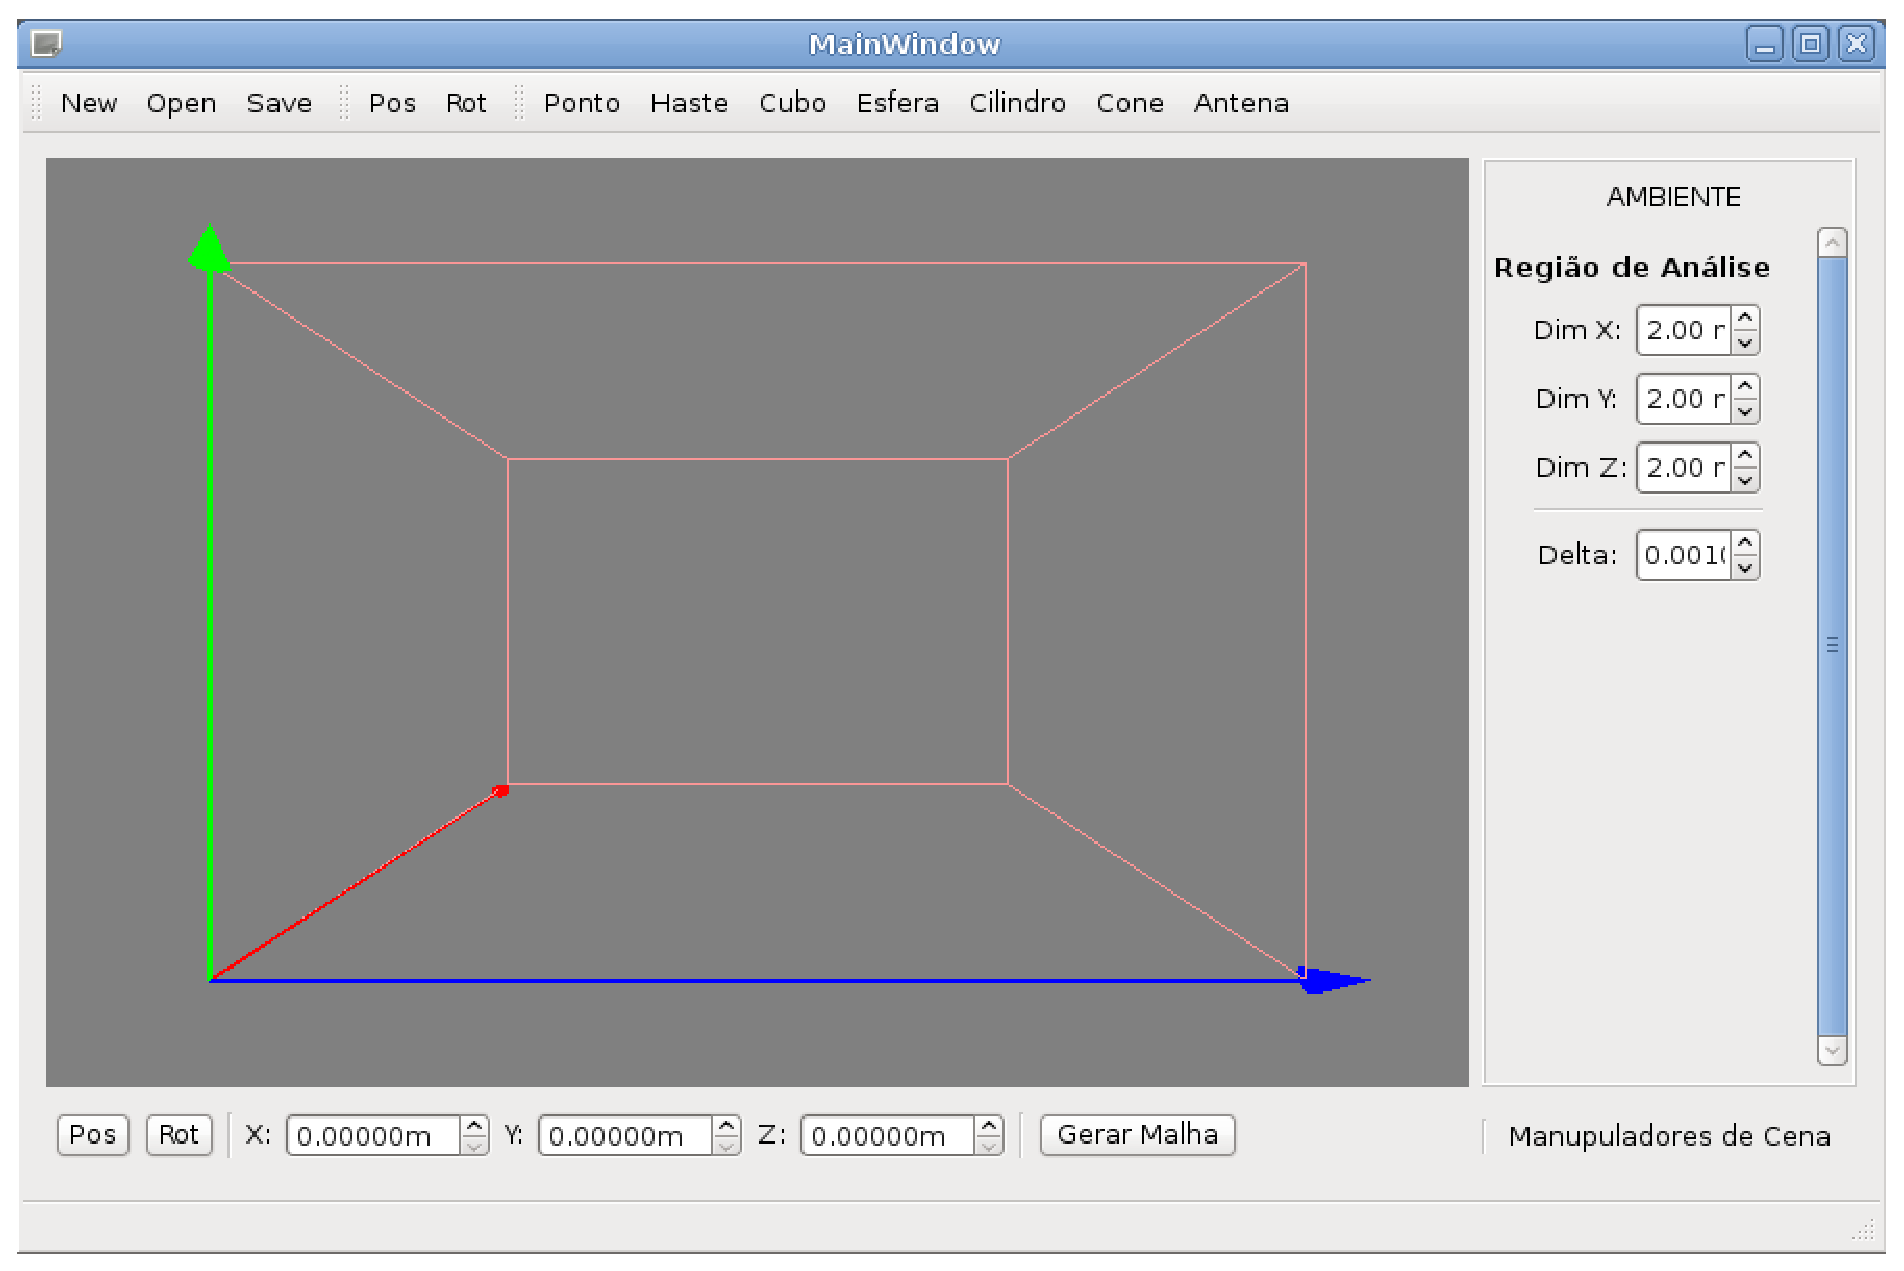
\includegraphics[scale = 0.4]{layout}
	\caption{Layout interface.}
	\label{fg:layout}
\end{figure}

Na barra superior, Figura~\ref{fg:barra_s}, encontramos primeiramente o botão \textit{New}, o qual ativará uma nova cena irrlicht. Quando pressionado ativara uma janela(Figura~\ref{fg:dados_r}) que requisitará os dados necessários para criação da região de análise, tais como dimensão $x$, $y$, $z$ e o valor do $delta$(dimensão da célula de Yee). Em seguida vem o botão \textit{Open}, que carrega uma cena anterior caso tenha já exista alguma salva. Depois dele temos o botão \textit{Save}, que salva a cena atual em uma arquivo chamado \textit{Map.in}, que contem todas as características dos objetos(dimensões, tipo e parâmetros de material) assim como suas posições.\\

\begin{figure}[ht!]
	\centering
	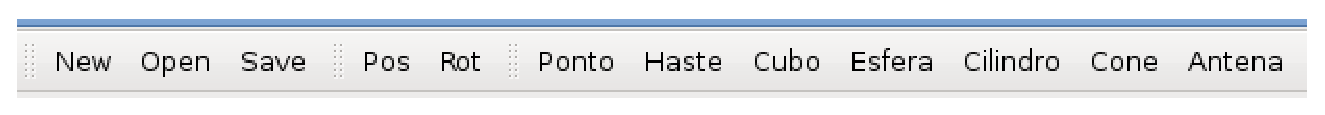
\includegraphics[scale = 0.4]{barra_s}
	\caption{Barra Superior interface.}
	\label{fg:barra_s}
\end{figure}
\begin{figure}[ht!]
	\centering
	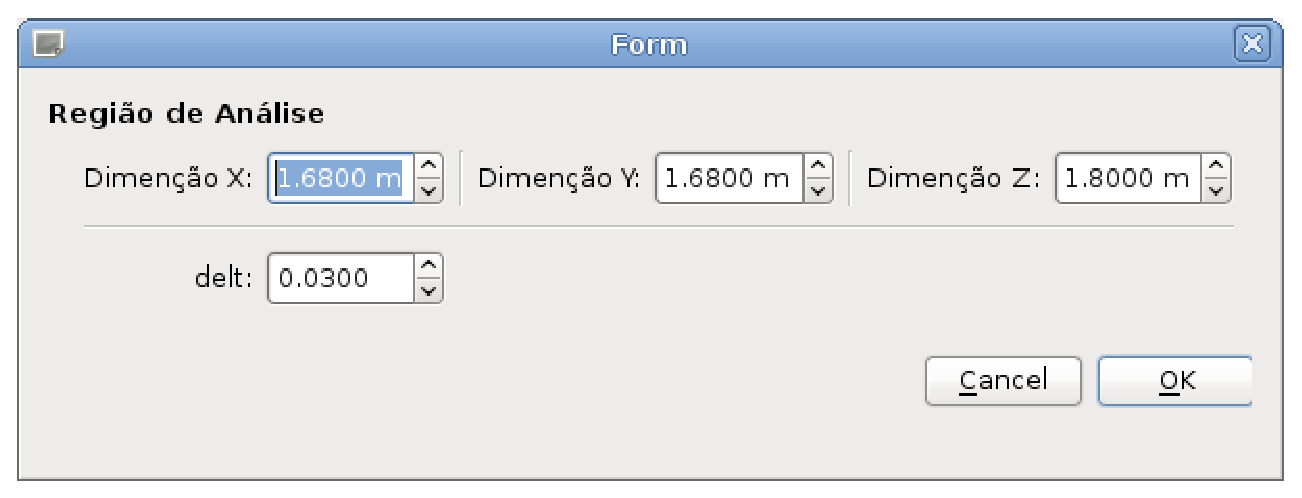
\includegraphics[scale = 0.4]{dados_r}
	\caption{Janela com as caracteristica da região de análise.}
	\label{fg:dados_r}
\end{figure}

Seguindo encontramos os botões \textit{Pos} e \textit{Rot}, os quais quando pressionados mostram o posicionamento e ângulos de rotação dos objetos selecionados respectivamente. Logo em seguida temos os criadores de objetos básico da interface, que são \textit{Ponto},\textit{Haste}, \textit{Cubo}, \textit{Esfera}, \textit{Cilindro}, \textit{Cone} e por fim \textit{Antena}. Quando ativados criam o objeto desejado com os parâmetros especificados, assim como sua posição.\\

A janela da cena, Figura~\ref{fg:janela_c} é onde visualizamos nosso universo virtual. O painel lateral, Figura~\ref{fg:painel_l} é onde encontramos as características como dimensão e parâmetros manterias do objeto selecionado ou criado.\\

\begin{figure}[ht!]
	\centering
	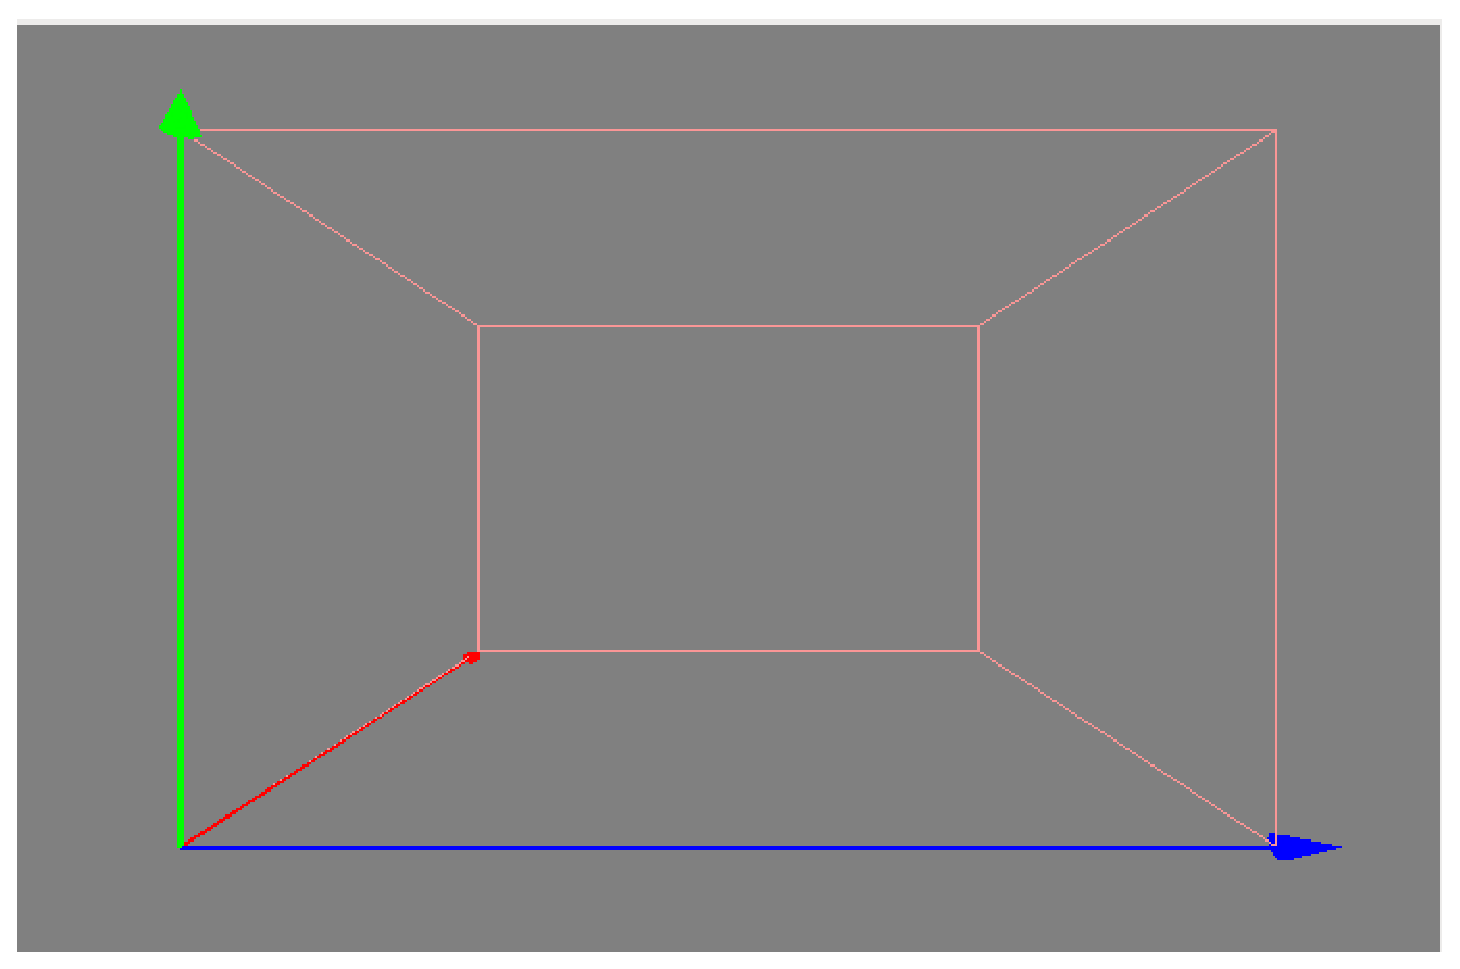
\includegraphics[scale = 0.4]{janela_c}
	\caption{Janela da Cena.}
	\label{fg:janela_c}
\end{figure}
\begin{figure}[ht!]
	\centering
	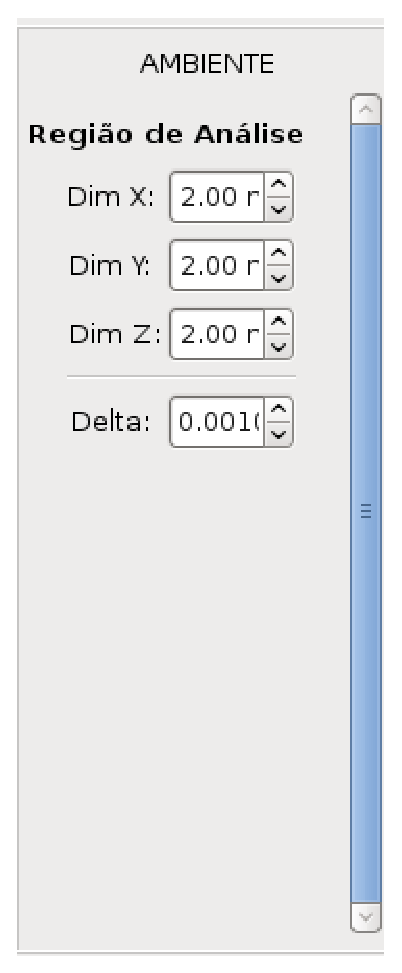
\includegraphics[scale = 0.4]{painel_l}
	\caption{Painel lateral dos parâmetros da região de análise.}
	\label{fg:painel_l}
\end{figure}

Na parte inferior da interface(Figura~\ref{fg:barra_i}) encontram-se os botões \textit{Pos} e \textit{Rot}, que têm as mesmas funcionalidades dos já sitados da barra superior. Assim como a coordenada do objeto selecionado($X$, $Y$ e $Z$). E por fim esta o botão \textit{gerar Malha}, o qual tem a função de gerar a malha compatível com o simulador LANE-SAGS.

\begin{figure}[ht!]
	\centering
	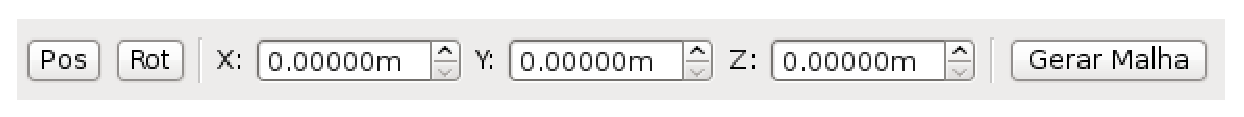
\includegraphics[scale = 0.4]{barra_i}
	\caption{Barra inferior da interface.}
	\label{fg:barra_i}
\end{figure}

\section{Funcionalidades}
	\subsection{Eventos de Mouse e Teclado}
	Tanto o irrlicht quanto o a biblioteca qt têm suporte a eventos de mouse e teclado. Todavia, o evento de mouse é visto e realizado de forma distinta. Então apareceu a necessidade de criação de um tipo de "comunicador" que "traduzisse" esse evento entres esses mundos diferentes.\\
	
	Na interface esse "comunicador" basicamente pegar as informações de mouse da janela do qt e envia de forma traduzida para o motor gráfico irrlicht. São basicamente três métodos do qt que foram modificados: mouseMoveEvent(), mousePressEvent() e mouseReleaseEvent().\\
	
	Já o evento de teclado não foi necessário o uso do "comunicador", pelo fato de não haver necessidade usarmos esse tipo de evento no irrlicht. Foram criados vários atalhos de teclado para facilitar a manipulação e navegação na cena, listados na tabela a seguir:
	
\begin{center}
\begin{tabular}{|l|l|}
    \hline
	Atalho & Funcionalidade \\ \hline
	Shift+O &  Afastamento\\ \hline
	Shift+P &  Aproximação\\ \hline
	W & Focaliza objeto selecionado\\ \hline
	C & Clona objeto selecionado(duplica)\\ \hline
	R & Remove objeto selecionado \\ \hline
	1 & Muda para camera frente \\ \hline
	2 & Muda para camera lateral esquerda \\ \hline
	3 & Muda para camera lateral direita \\ \hline
	4 & Muda para camera traseira \\ \hline
	5 & Muda para camera topo \\ \hline
	6 & Muda para camera base \\ \hline
	M + X & Permite movimentação de objeto selecionado no eixo X com o mouse \\ \hline
	M + Y & Permite movimentação de objeto selecionado no eixo Y com o mouse \\ \hline
	M + Z & Permite movimentação de objeto selecionado no eixo Z com o mouse \\ \hline
	Shift + A & Permite movimentação de objeto selecionado nos eixos X e Y com o mouse \\ \hline
	Shift + B & Permite movimentação de objeto selecionado nos eixos X e Z com o mouse \\ \hline
	Shift + C & Permite movimentação de objeto selecionado nos eixos Y e Z com o mouse \\ \hline
	Shift + D & Permite movimentação de objeto selecionado nos eixos X, Y e Z com o mouse \\ 
    \hline
\end{tabular}
\end{center}
	
	\subsection{Colisão}
	O evento de colisão foi feito baseado na teoria de jogos. Existem vários tipos de colisão, porém a utilizada nesse trabalho foi a de resposta por reta. Seu funcionamento é bem simples, cria-se uma reta imaginária na cena onde seu ponto de origem é a câmera e seu fim esta localizado em um ponto bastante distante ao inicial. Esse ponto final acompanha o movimento do mouse. Então quando clica-se em um dado ponto do universo criado na interface é disparado o evento de colisão o qual retorna {nó}\footnote{Objeto selecionado} selecionado. \\
	
	Mas isso só vale quando o há um objeto na coordenada selecionada sendo ele selecionável. No caso de se clicar em um dos gizmos\footnote{Orientadores de eixo, gizmo verde(representa o eixo $y$), gizmo azul(representa o eixo $x$) e gizmo vermelho(representa o eixo $z$)} da região de análise, por exemplo, o evento de colisão retornará um objeto vázio, apesar de o gizmo ser um objeto normal ele foi configurado como não selecionável assim fazendo com que mesmo que a reta colida com ele o resultado será nulo. A Figura~\ref{fg:colision} mostra a ocorrência desse evento na interface, como pode-se observar o objeto selecionado é pintado na sua forma armada ou wireframe para diferenciar dos não selecionados.
	
\begin{figure}[ht!]
	\centering
	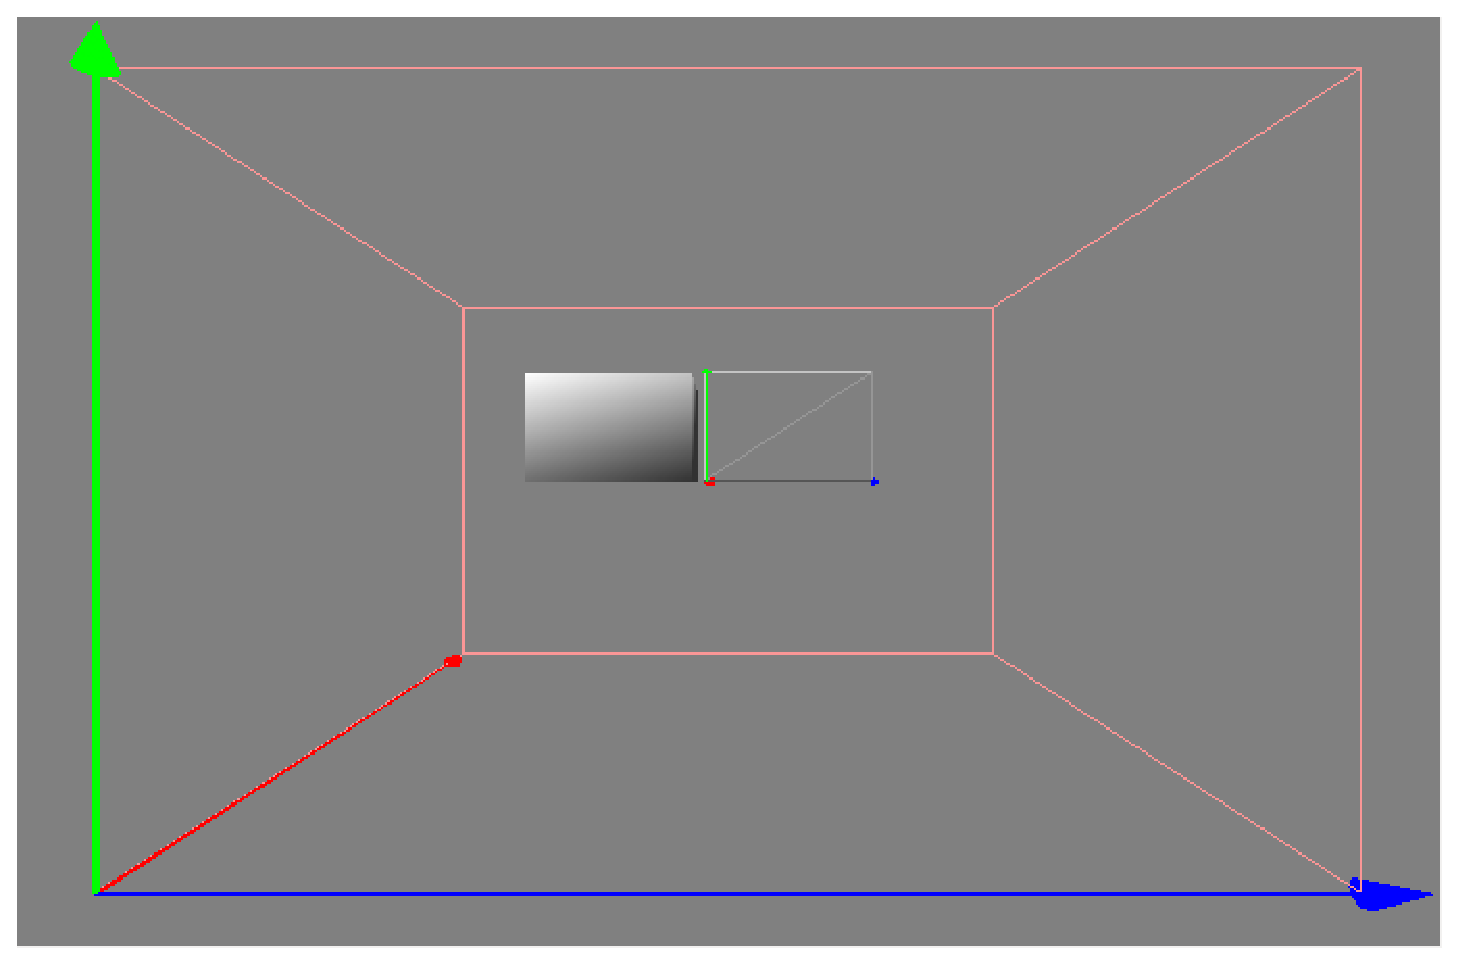
\includegraphics[scale = 0.4]{colision}
	\caption{Ilustração do evento de colisão com o objeto cubo.}
	\label{fg:colision}
\end{figure}

	\subsection{Visualizações}
	Ter vários ângulos de visualização é fundamental quando esta se modelando um ambiente 3D, principalmente quando vamos usá-lo para simulação de ondas eletromagnéticas pelo fato de qualquer erro deixado na estrutura poderá alterar no resultado final. Para sanar esse problema, o software confeccionado nesse projeto, permitir visualizar a região de análise por seis câmeras diferentes: frente(padrão), lateral esquerda, lateral direita, por trás, topo e base. 
	
	\subsection{Aproximação e Afastamento}
	É uma característica importante da interface criada nesse projeto. Ela permite se aproximar(através do atalho de teclado Shift+P) e afastar(por meio de Shift+O) conforme desejarmos de uma objeto que se encontra dentro da região de análise. Assim permitindo navegar pelo cenário virtual criado, podendo alterar, remover e duplicar objetos conforme desejado. Uma outra especificação dessa propriedade esta associada ao fato de quando temos um objeto selecionado. Se pressionarmos a tecla W a câmera ira ter como foco esse objeto. Para melhor entendimento a Figura~\ref{fg:nor} mostra a visualização de um objeto sem alteração de foco da câmera e distancia, já a Figura~\ref{fg:afas} mostra a visualização após um determinado afastamento e por fim as Figuras~\ref{fg:apr} e \ref{fg:w} mostram a aproximação normal e a por seleção.
	
\begin{figure}[ht!]
	\centering
	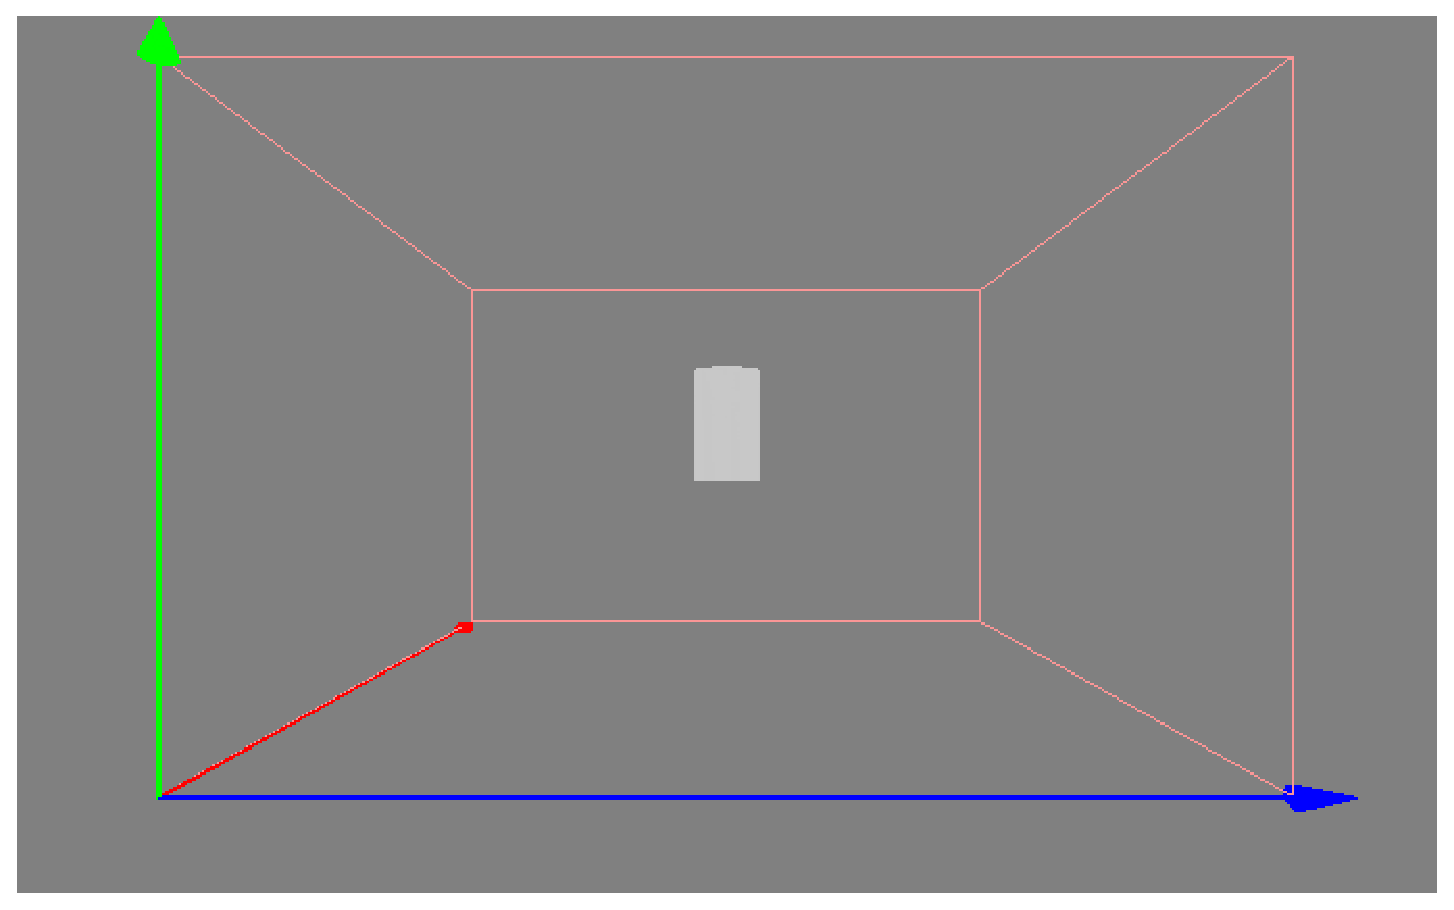
\includegraphics[scale = 0.4]{nor}
	\caption{Visualização de objeto cilindro sem aproximação, afastamento ou mudança de foco da câmera.}
	\label{fg:nor}
\end{figure}
\begin{figure}[ht!]
	\centering
	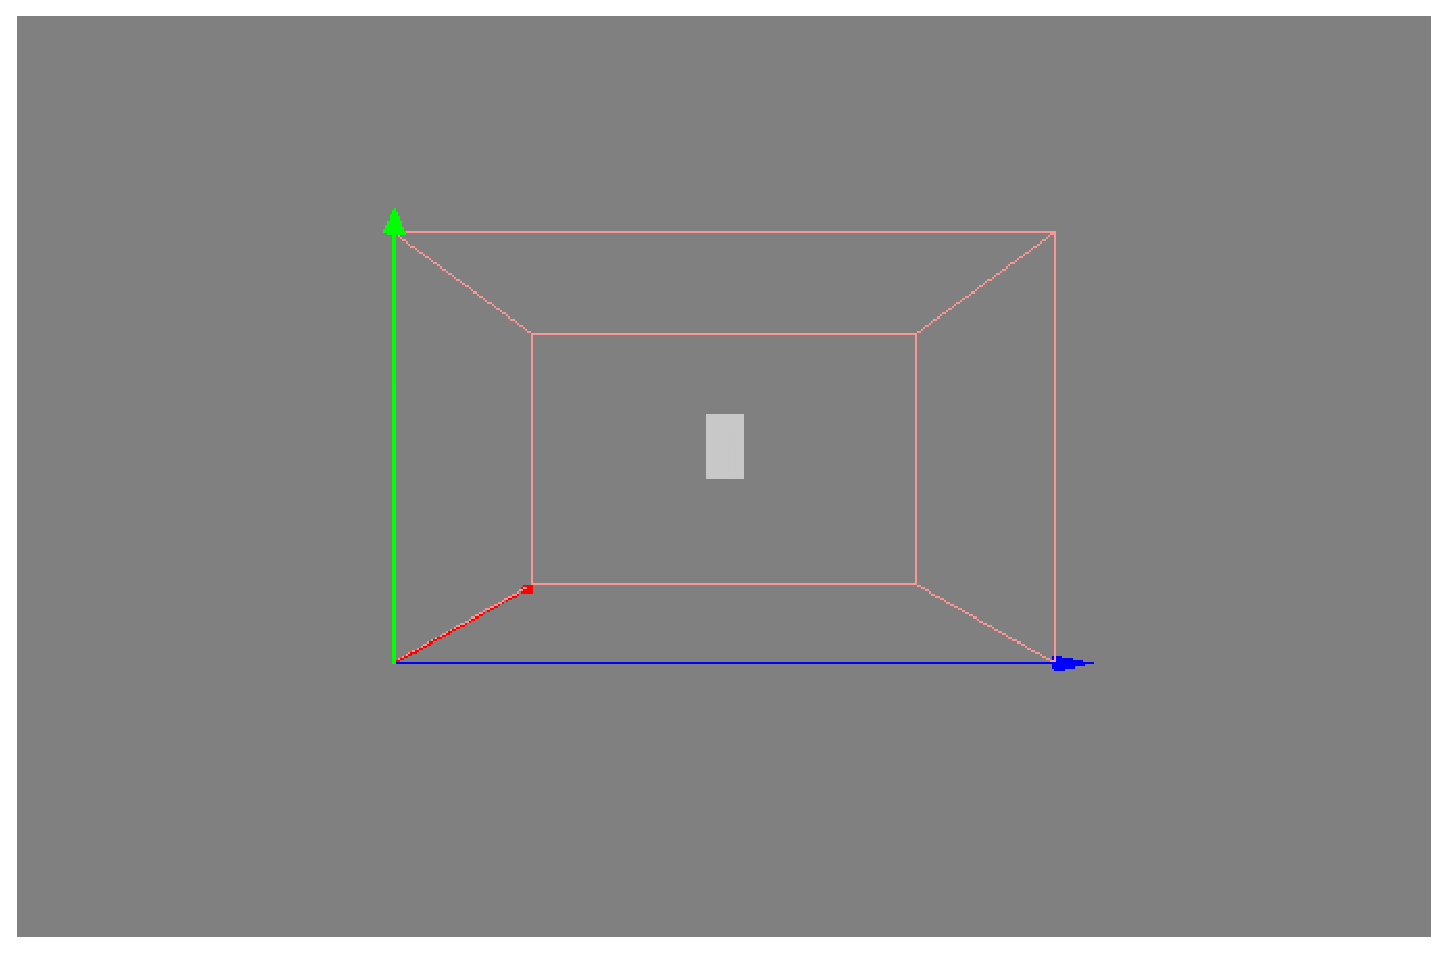
\includegraphics[scale = 0.4]{afas}
	\caption{Visualização de objeto cilindro com afastamento.}
	\label{fg:afas}
\end{figure}
\begin{figure}[ht!]
	\centering
	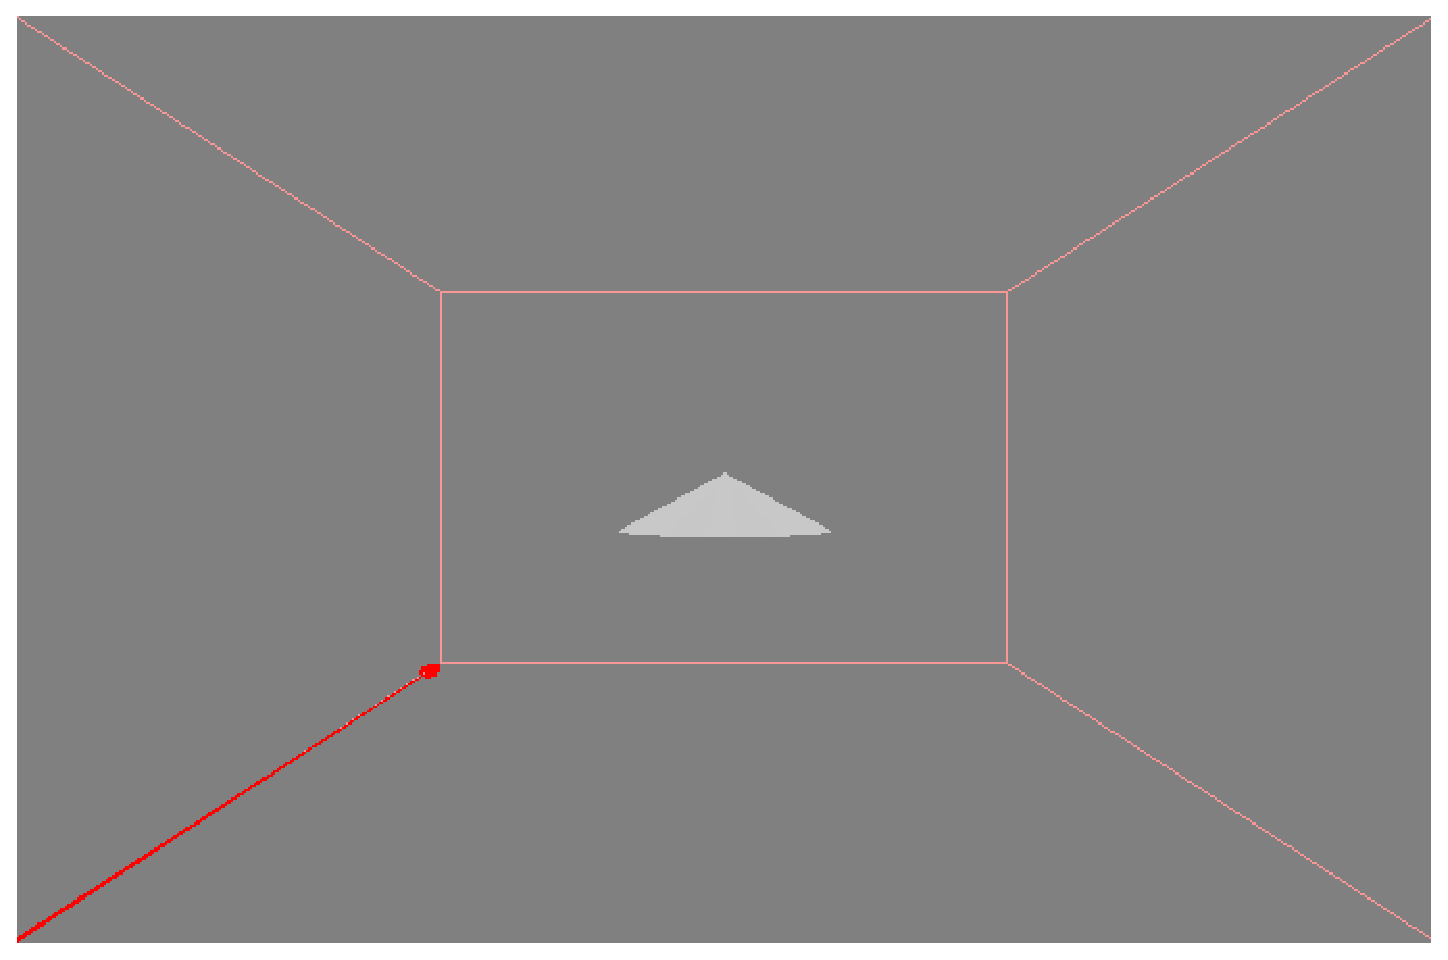
\includegraphics[scale = 0.4]{apr}
	\caption{Visualização de objeto por aproximação normal(sem mudança de foco).}
	\label{fg:apr}
\end{figure}
\begin{figure}[ht!]
	\centering
	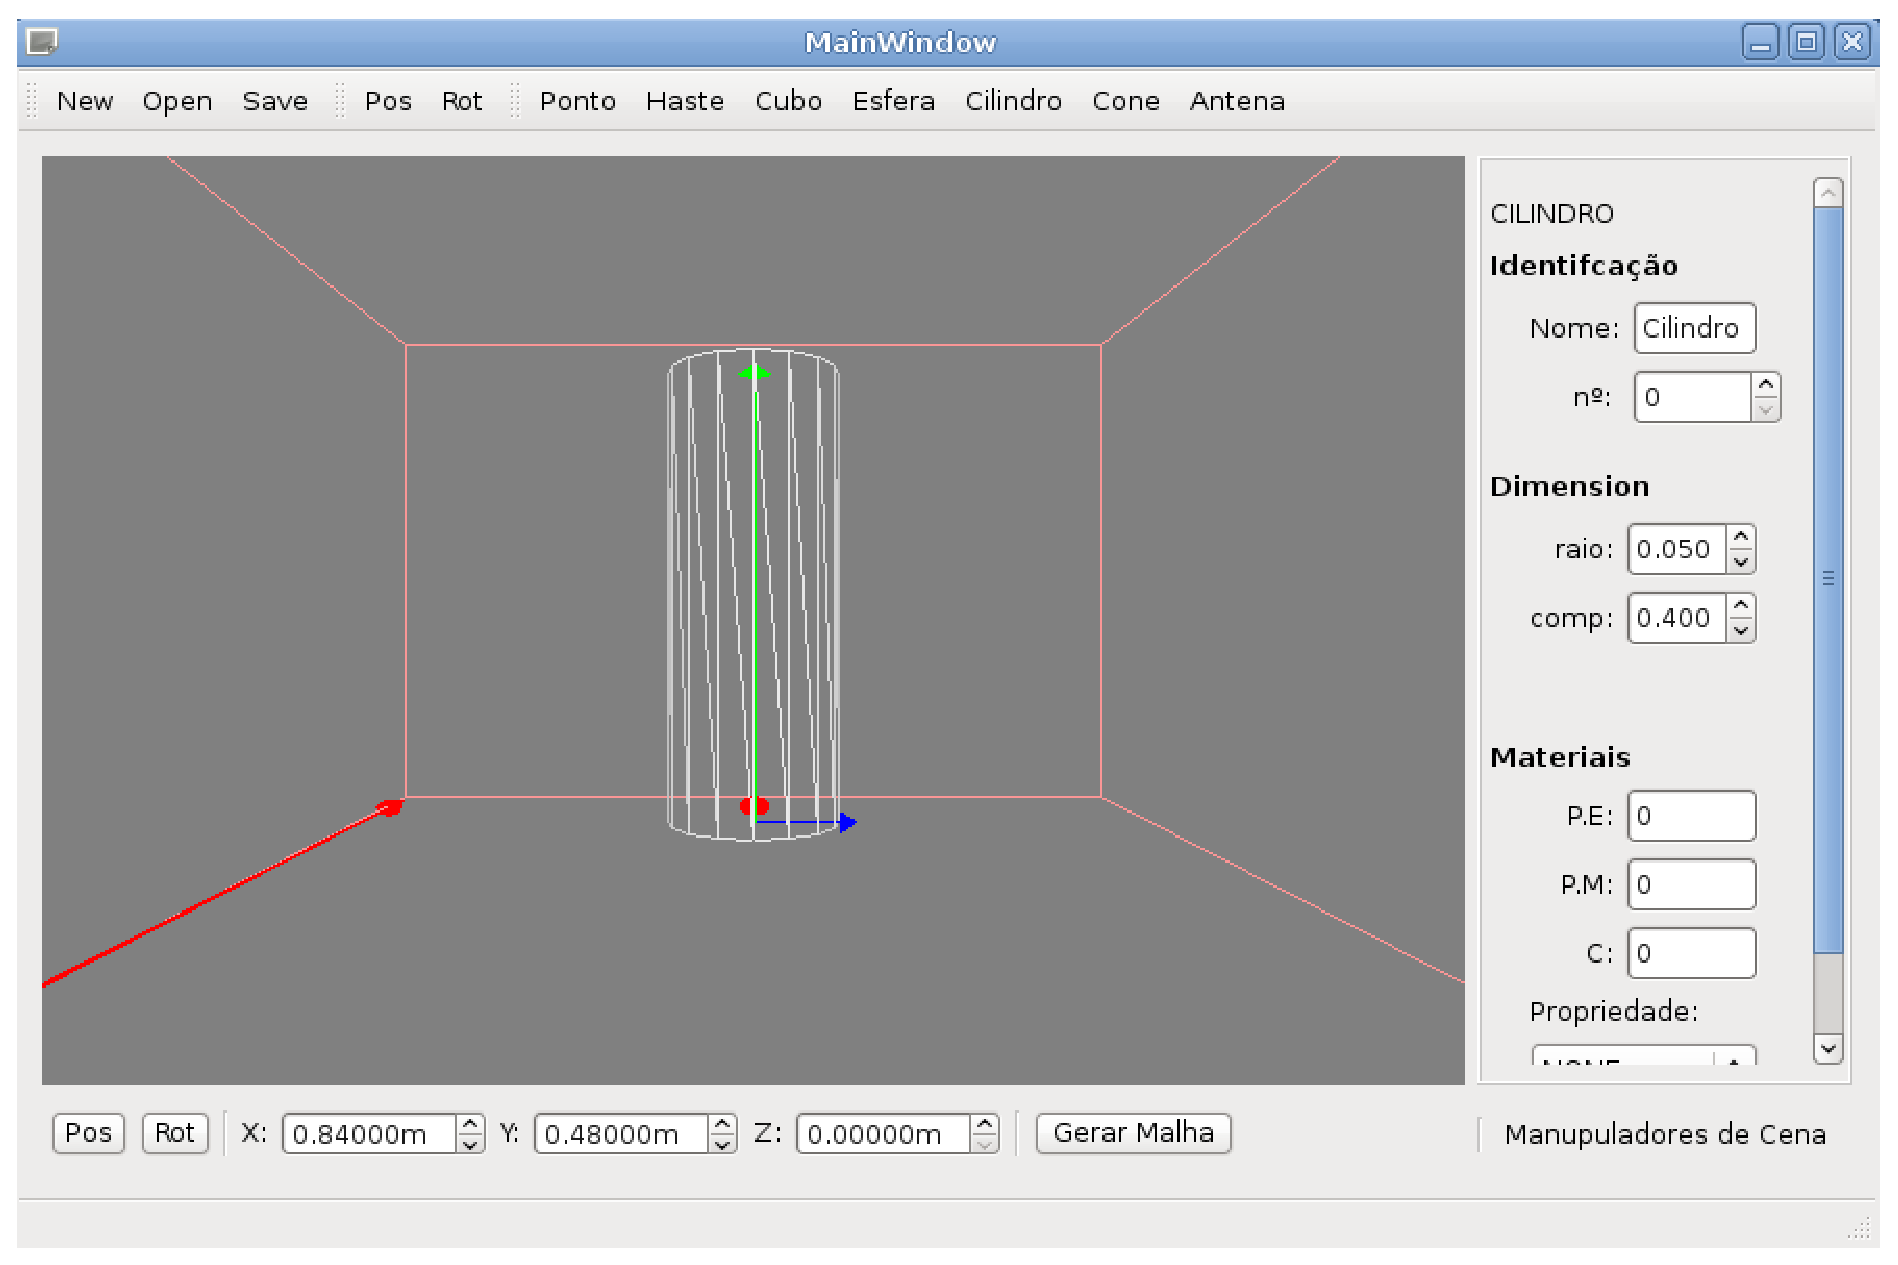
\includegraphics[scale = 0.4]{w}
	\caption{Focalização de objeto selecionado através do atalho de teclado W.}
	\label{fg:w}
\end{figure}

	\subsection{Remoção e Duplicação de Objetos}
	Nesse trabalho houve a necessidade criação de um mapa de objetos, pelo fato do irrlicht não permitir acesso ao seu array de objetos criados na cena. Dessa forma, qualquer alteração, remoção ou clonagem feita em um objeto na cena terá correspondência no mapa de \textit{nós} gerenciado pela interface. Com isso, quando removemos um objeto criado na região de análise, ele também será removido do mapa. As Figuras~\ref{fg:b_r} e \ref{fg:a_r} mostram a antes e depois de removermos um \textit{nó} do nosso universo virtual. \\
	
	O mesmo ocorre quando deseja-se duplicar um objeto, uma vez que isso ocorra o mapa receberá mais um \textit{nó} com as mesmas característica do selecionado. Esse evento esta representado pelas Figuras~\ref{fg:b_c} e \ref{fg:a_c}.
	
\begin{figure}[ht!]
	\centering
	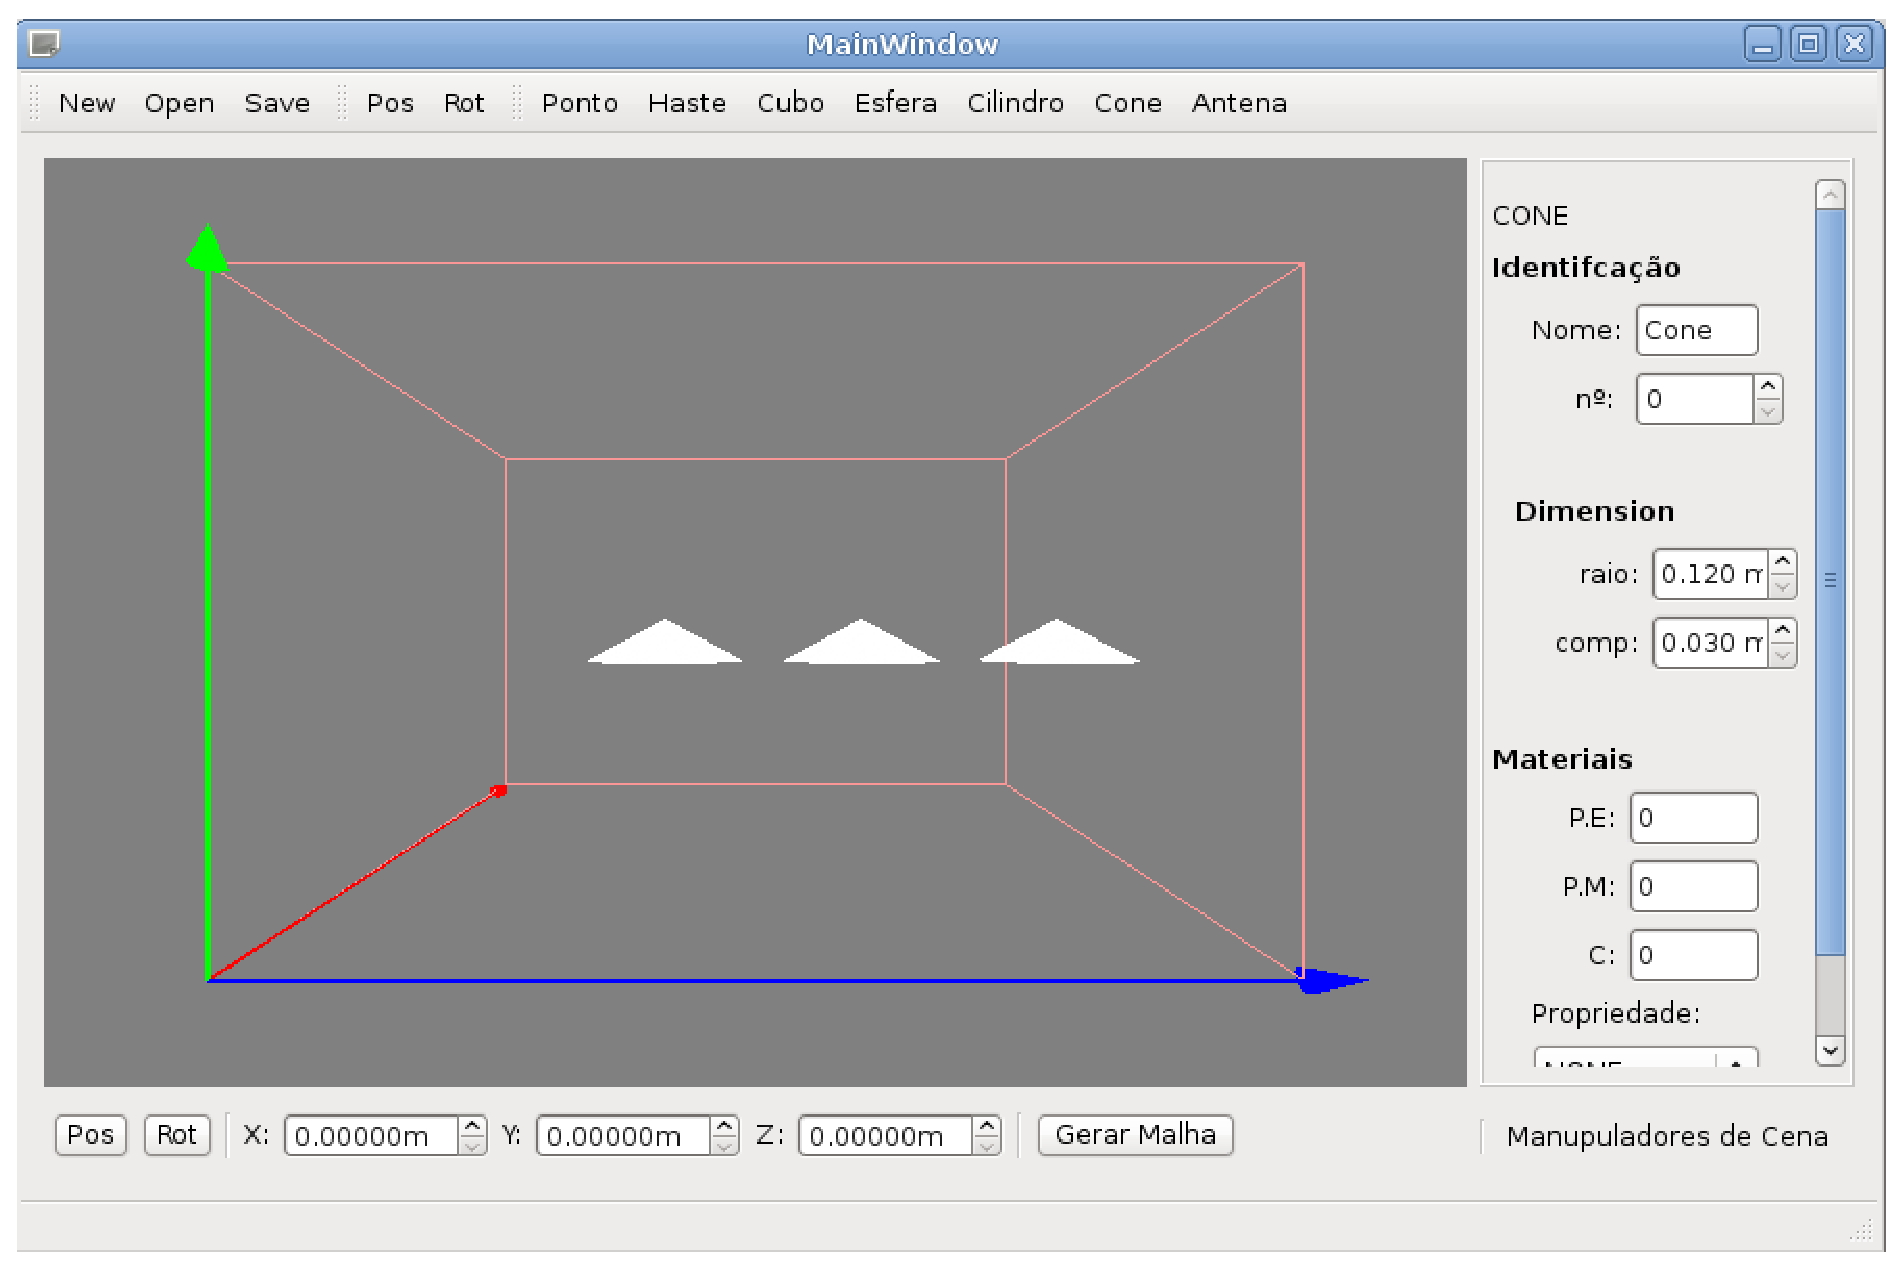
\includegraphics[scale = 0.4]{b_r}
	\caption{Antes da remoção.}
	\label{fg:b_r}
\end{figure}
\begin{figure}[ht!]
	\centering
	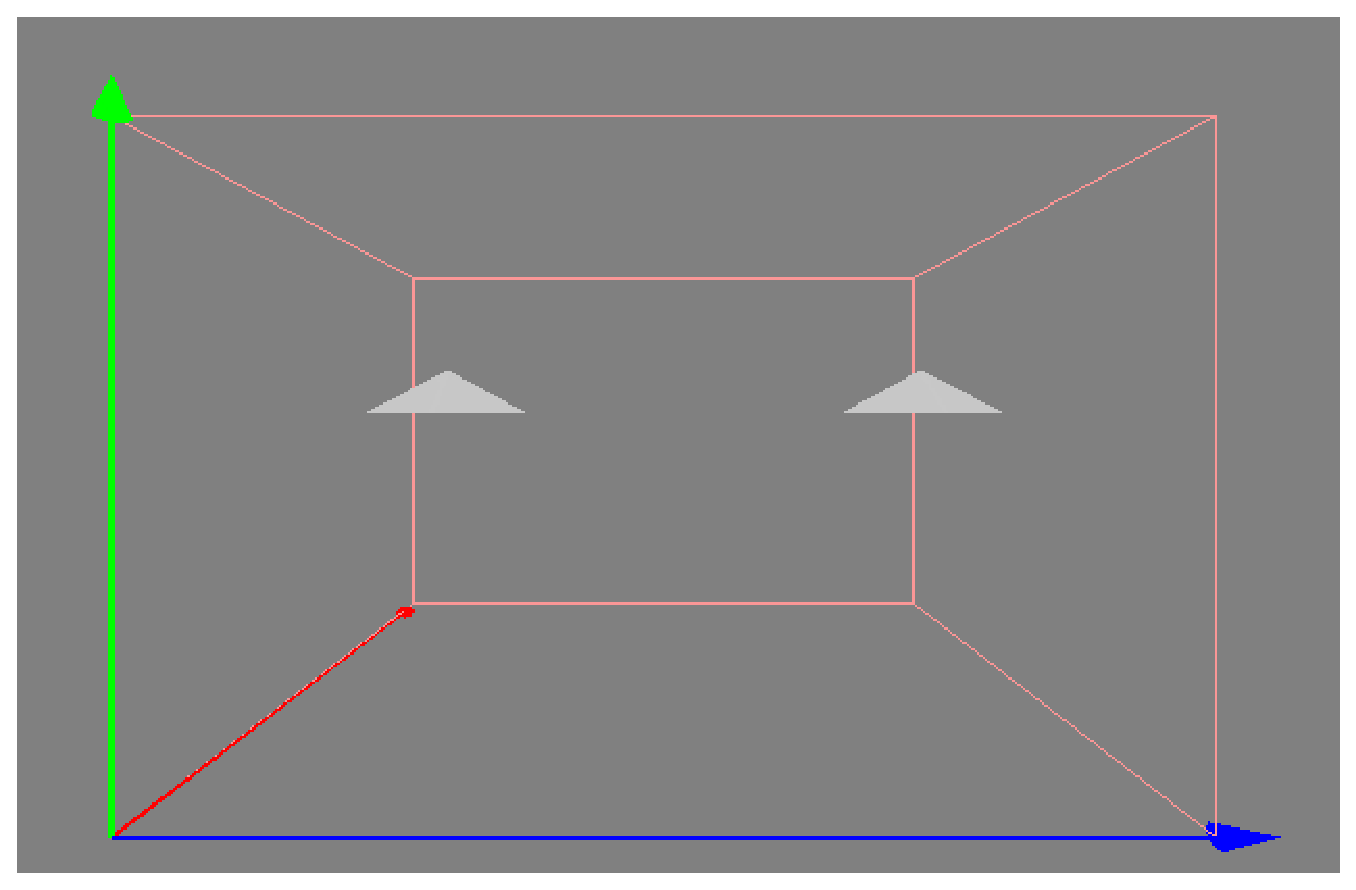
\includegraphics[scale = 0.4]{a_r}
	\caption{Depois da remoção.}
	\label{fg:a_r}
\end{figure}
\begin{figure}[ht!]
	\centering
	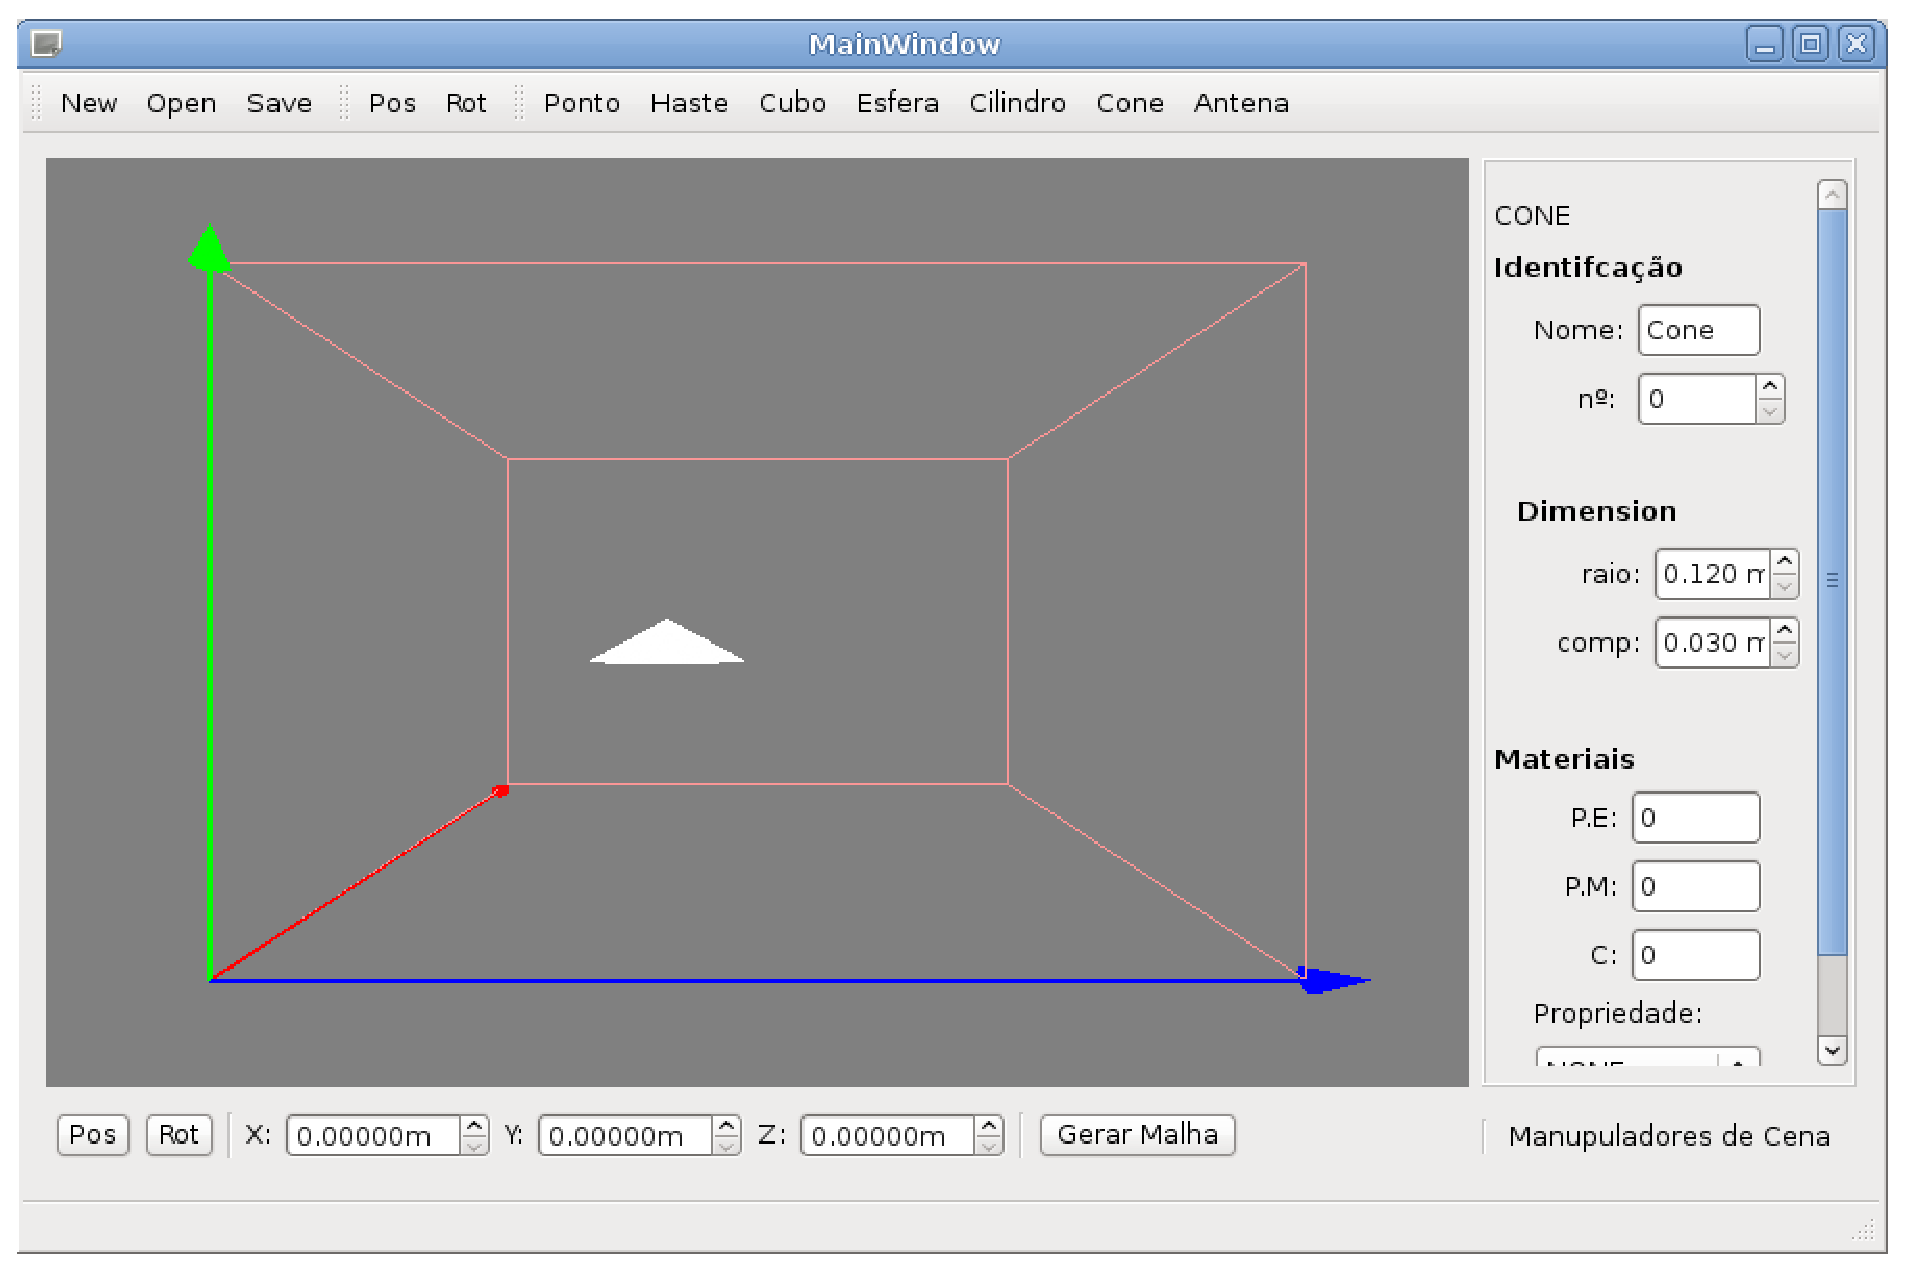
\includegraphics[scale = 0.4]{b_c}
	\caption{Antes da duplicação do objeto cone.}
	\label{fg:b_c}
\end{figure}
\begin{figure}[ht!]
	\centering
	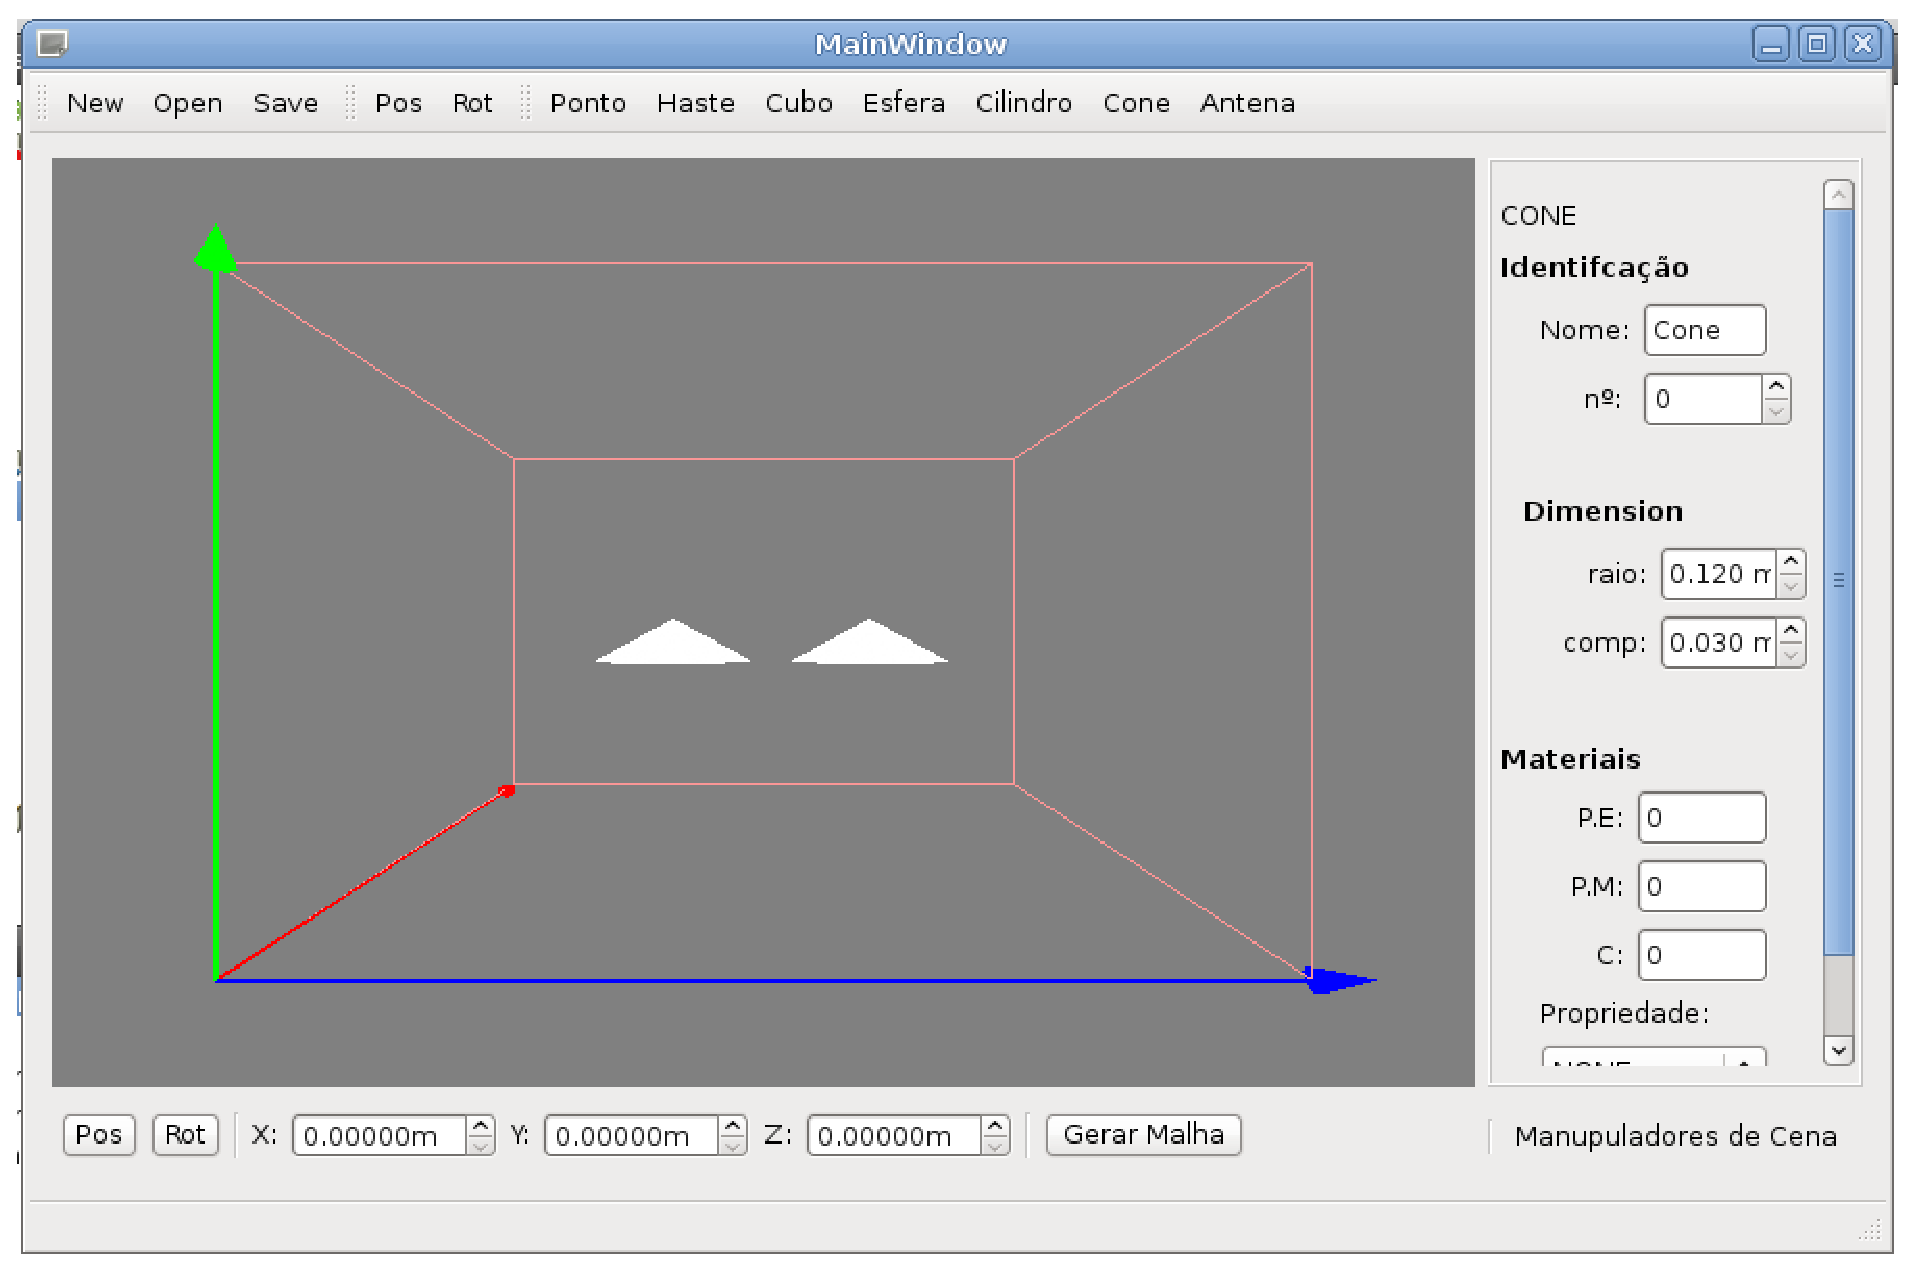
\includegraphics[scale = 0.4]{a_c}
	\caption{Depois da duplicação do objeto cone.}
	\label{fg:a_c}
\end{figure}

	\subsection{Conexão com o LANE-SAGS}
Como dito anteriormente a interface aqui produzida cria ambientes tridimensionais que podem ser utilizados em simulações em FDTD, porém, o mesmo não executa as simulações. Para que isso ocorra, é necessário o acoplamento desse ambiente com outro software que torne isso possível, o que é realizado através de arquivos de entrada e saída.\\
	
Esse software produzido nesse trabalho possui um sistema genérico de geração de arquivos de saída. Este sistema reconhece os objetos criados pela interface e cria uma representação destes objetos a partir de um conjunto de prismas retangulares. Cada prisma do conjunto representativo possui as características físicas de $\epsilon$(Permissividade Elétrica), $\sigma$(Condutividade Elétrica) e $\mu$(Permeabilidade Magnética) do objeto que representa.\\

A sequência de prismas representativos é gravada em um arquivo de saída chamado bd.in, compatível com o simulador LANE-SAGS. Cada prisma da sequência tem suas coordenadas e características físicas armazenados da seguinte forma: célula inicial $X$, célula final $X$, célula inicial $Y$, célula final $Y$, célula inicial $Z$, célula final $Z$,$\epsilon$, $\sigma$ e $\mu$; Além deste arquivo, contendo a sequência de prismas representativo dos objetos, é gerado um segundo arquivo chamado \textit{simconf.in} contendo as informações referentes às: dimensões das células de Yee (em metros) e a dimensão em células do Espaço Delimitador (região de análise).\\

Com a conexão realizado, basta adicionar alguns parâmetros como: antenas, planos de visualização, fonte, corrente; para então simular o ambiente. O diagrama mostrado na Figura \ref{fg:c_sags}, ilustra o processo de execução de uma simulação utilizando os dois softwares.
\begin{figure}[ht!]
	\centering
	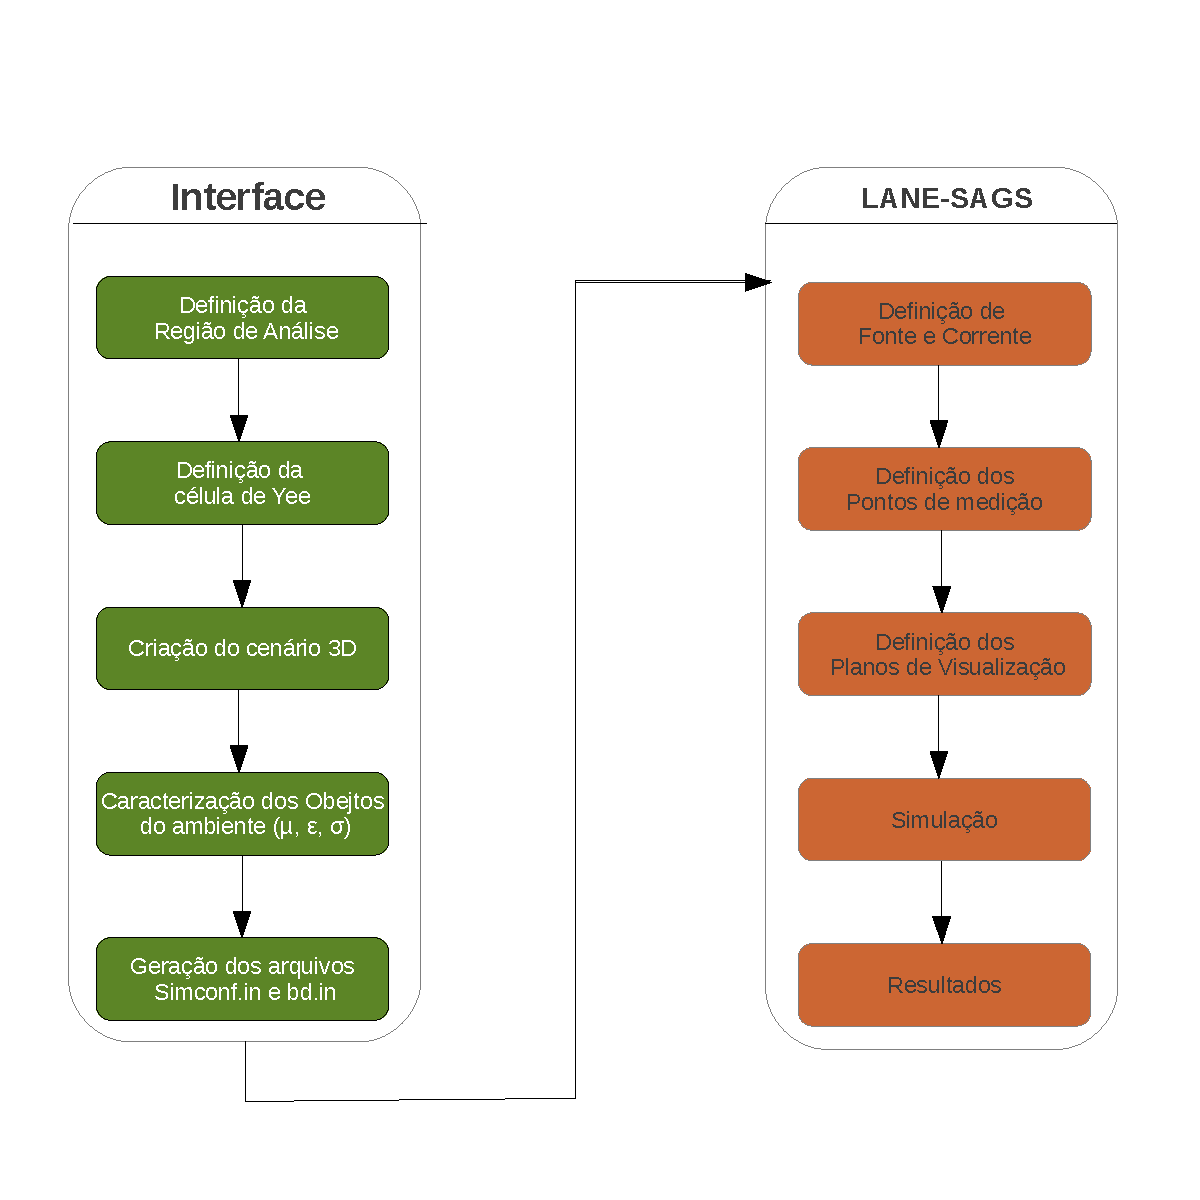
\includegraphics[scale = 0.4]{c_sags}
	\caption{Diagrama de conexão com o LANE-SAGS.}
	\label{fg:c_sags}
\end{figure}


\chapter{Aplicação e Resultados}
%Com a finalidade de validar a interface, foi construído um AV apartir da caracteristicas de um ambiente real(escritório), com planta baixa ilustrada na Figura~\ref{fg:planta_baixa}. Também foram modelados os objetos presentes nessa cenário real, como : computadores, monitores, bancadas, divisórias de vidro e porta.\\

\begin{figure}[ht!]
	\centering
	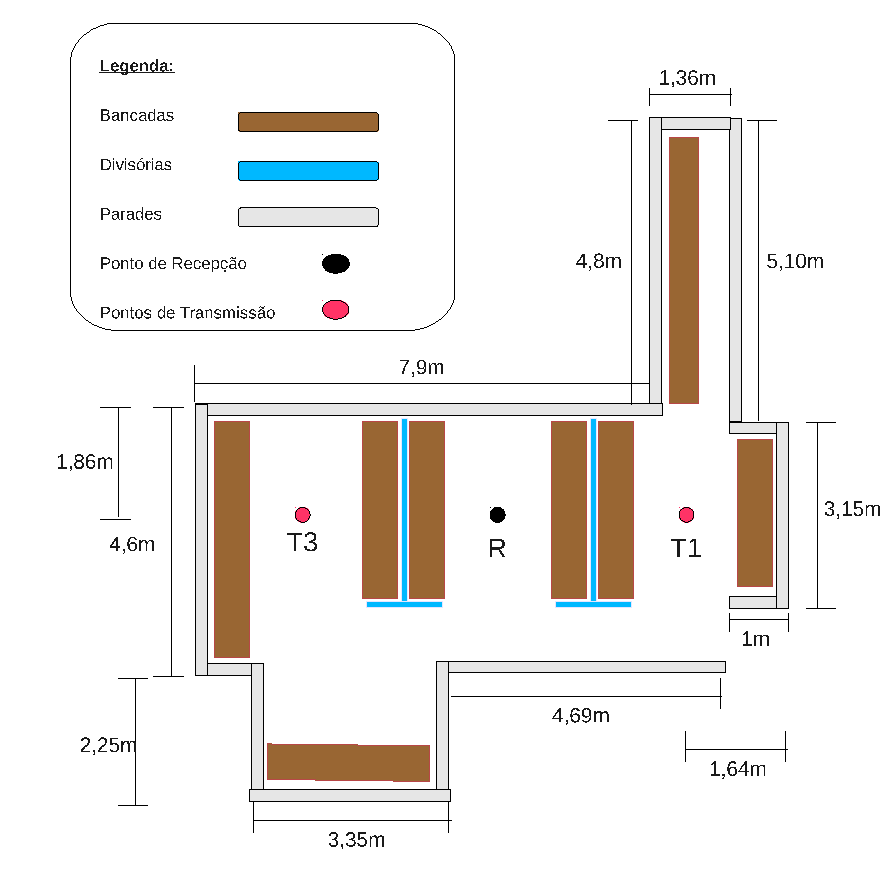
\includegraphics[scale = 1]{planta_baixa}
	\caption{Planta baixa do escritório modelado usando a interface.}
	\label{fg:planta_baixa}
\end{figure}

Esperimentalmente, posde-se observar o comportamento da propragação do sinal de uma antena nesse escritório. 

Alguns desse objetos estão dispostos em alturas diferentes em relação ao piso. As bancadas e o teto estão a uma altura de 0,75 metros e 2,73 metros, respectivamente.\\

Como resultado da modelagem usando a interface, obeteve-se a estrutura mostrada na Figura(colocar figura estrutura da interface). A disposição dos seus objetos seguiu a posicionamento real dos mesmos no momento das medições.
%\begin{figure}[ht!]
%	\centering
%	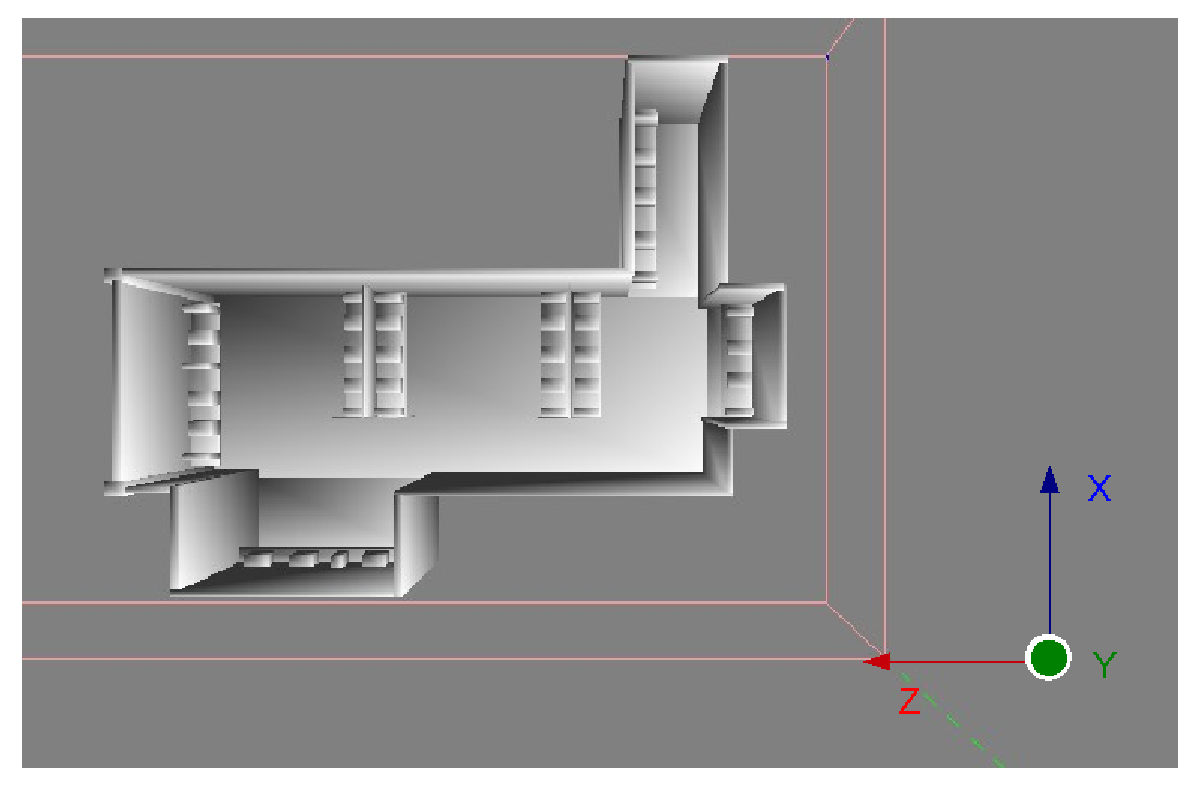
\includegraphics[scale = 0.4]{ambiente}
%	\caption{Visão topo em pespectiva do ambiente construído através da interface.}
%	\label{fg:ambiente}
%\end{figure}

As especificações desse cenário, foram:
\begin{itemize}
\item \textit{Delta}(Tamanho da célula de Yee) utilizada foi de $0,003m$.
\item \textit{Região de Análise} com dimensões: $X$ = $15m$, $Y$ = $3m$ e $Z$ = $15m$.
\item \textit A lista das carateristicas físicas com seus respectivos matérias estam presentes na Tabela~\ref{tab:materiais}
\end{itemize}

\begin{center}
	\begin{tabular}{|l|l|l|l|l|}
	\hline
	Elementos dos Ambiente & Material & $\epsilon$ & $\sigma$ & $\mu$ \\ \hline
	Parede & Tijolo & 4 & 0,0135 & 1\\ \hline
	Teto & Gesso & 2,8 & 0,1533 & 1 \\ \hline
	Bancadas & Madeira & 1,8 & 0,011 & 1\\ \hline
	Monitores e Gabinetes & Metal & 5 & $valor$ & 1\\ \hline
	Divisórias & Vidro & 5 & $valor$ & 1 \\ \hline
	Piso & Concreto & 5 & 1 & 1 \\
	\hline
	\end{tabular}
	\label{tab:materiais}
\end{center}

%antena
Depois de ambiente ter sido montado, surguiu a necessidade de se introduzir a antena . Como a que foi usada na medição não tinha uma representação virtual, foi necessário criá-la. Com isso foram feitos alguns teste usando antenas dipolo, com o intuito de obeter a máxima aproximação do comportamento da antena real. \\

Para todos os modelos de antena foi ultizada uma fonte de tensão de trêm de pulsos normalizado, Figura~\ref{fg:fonte}, onde através da transforma de Fourier, pode-se observar se a mesma estava trabalhando na banda adequada. O resultado obtido foi o ilustrado na Figura~\ref{fg:fonte_f}.\\

A primeira antena feita foi um dipolo mostrado na figura~\ref{fg:antena_normal}

%\begin{figure}[ht!]
%	\centering
%	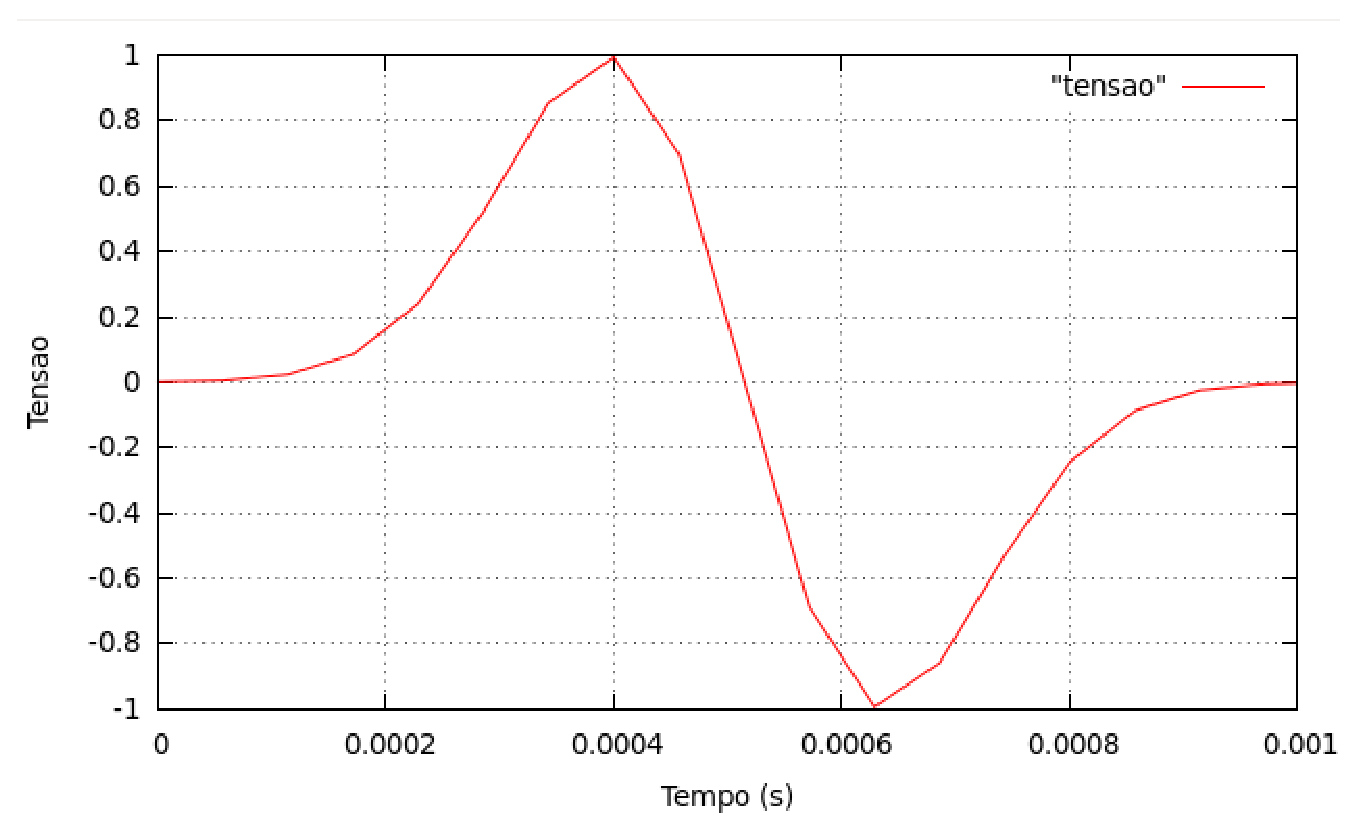
\includegraphics[scale = 0.4]{tensao}
%	\caption{Gráfico da fonte(trêm de pulsos).}
%	\label{fg:fonte}
%\end{figure}
%\begin{figure}[ht!]
%	\centering
%	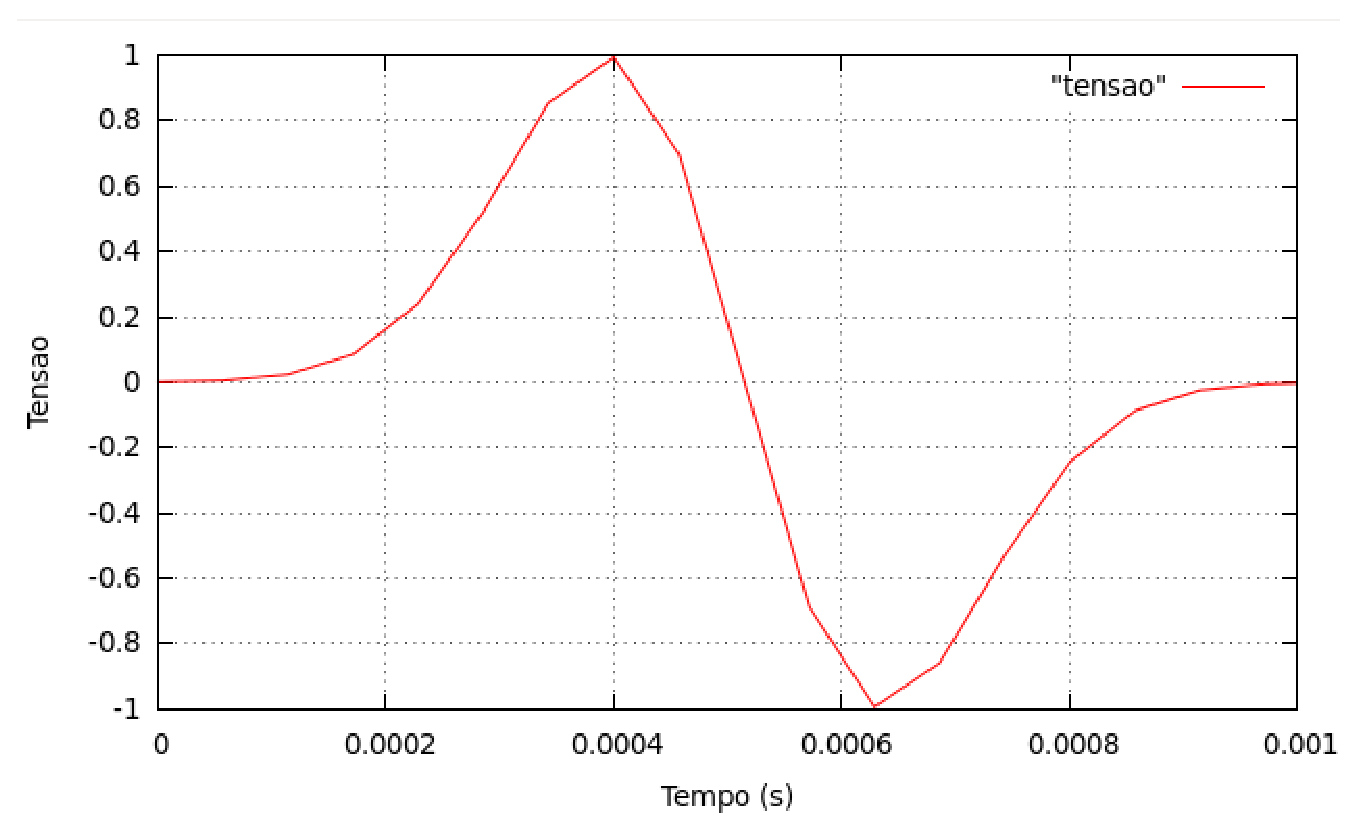
\includegraphics[scale = 0.4]{tensao}
%	\caption{Gráfico da fonte transformada de Fourier da fonte.}
%	\label{fg:fonte_f}
%\end{figure}

%\begin{figure}
%	\begin{subfigure}[b]{0.3\textwidth}
%			\centering
%			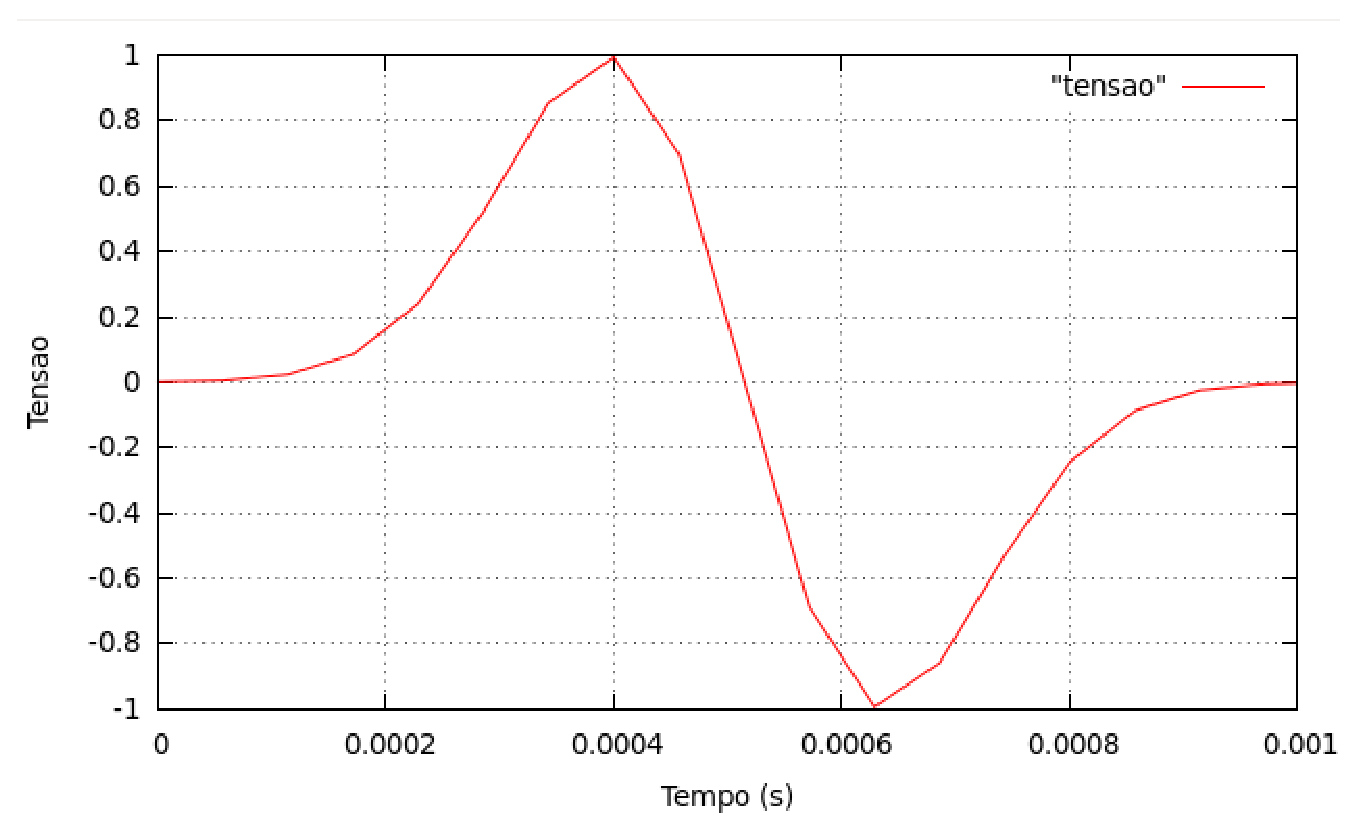
\includegraphics[width=\textwidth]{tensao}
%			\caption{Gráfico da fonte de tensão(trêm de pulsos).}
%			\label{fg:fonte}
%	\end{subfigure}%
%	~ %add desired spacing between images, e. g. ~, \quad, \qquad etc. 
%	  %(or a blank line to force the subfigure onto a new line)
%	\begin{subfigure}[b]{0.3\textwidth}
%			\centering
%			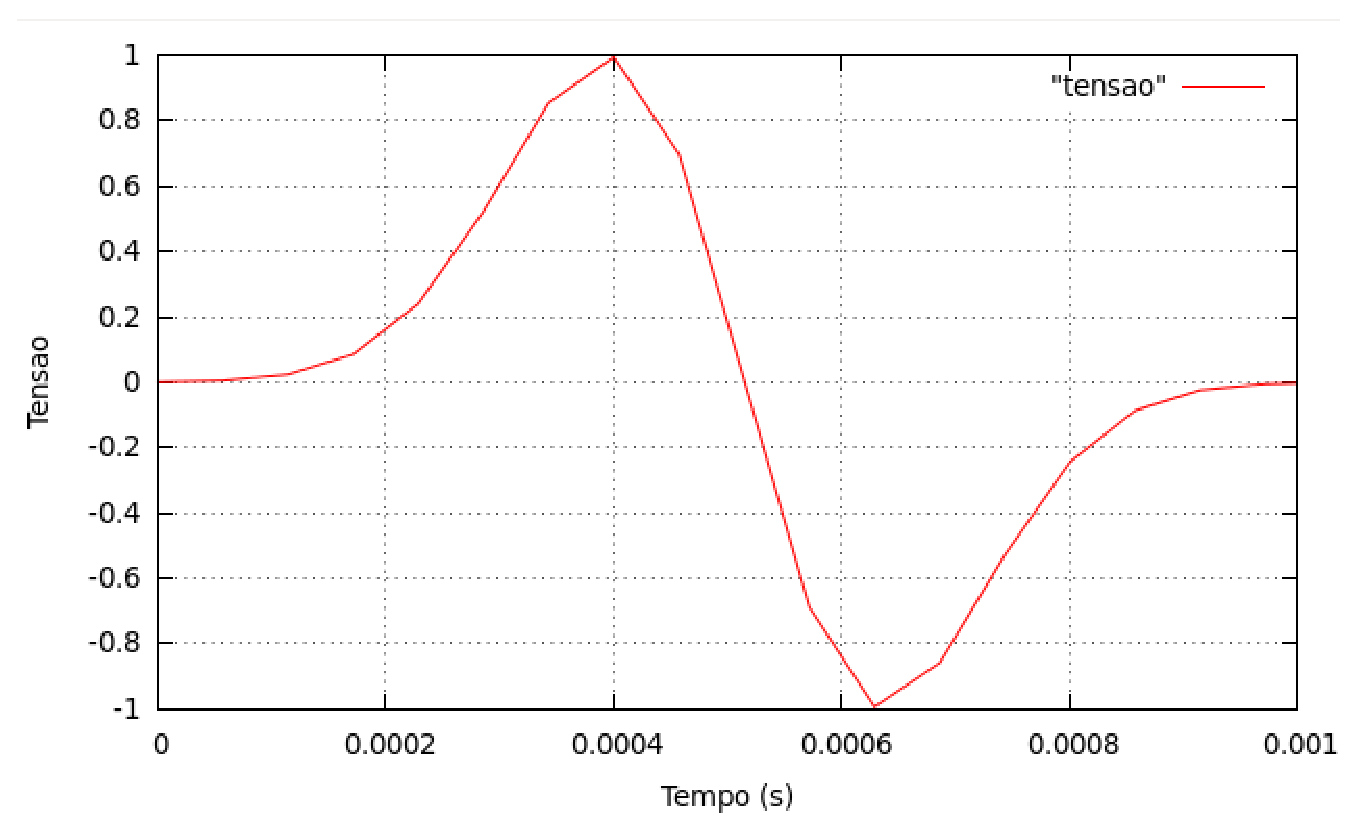
\includegraphics[width=\textwidth]{tensao}
%			\caption{Gráfico da transformada de Fourier da fonte (banda na qual esta trabalhando).}
%			\label{fg:fonte}
%	\end{subfigure}
%	~ %add desired spacing between images, e. g. ~, \quad, \qquad etc. 
%	  %(or a blank line to force the subfigure onto a new line)
%	\caption{Fonte da Antena}\label{fg:fonte_antena}
%\end{figure}





 Visto que o sua perda de retorno não foi satisfatória, foram feitas modificações em sua dimensão e por fim foi adicionado um  capacitor(Figura(colocar figura antena capacitor)). Com essas mudanças se obteve um antena com um comportamento parecido com o da real. Os gráficos de perda dessas duas construções esta ilustrado na Figura(colocar figura da perda)
%resultados


\chapter{Considerações Finais}
%Nesse trabalho foi desenvolvido um software de modelagem 3D que permite construir ambientes virtuais baseados nas caracteristicas dos reais. Ele se ultiza das tecnicas de modelagem mais usadas no mercado, além de também utilizar da teoria de grafo de cena. Possibilitando que o cenário nele desenvolvido simule a progação de ondas eletromagnéticas usando a método FDTD.\\

Um estudo de caso foi realisado, obtendo um resultado satisfatório que comprovou que tanto a modelagem quanto a conexão com o simulador LANE-SAGS funcionaram de forma desejada. Assim, mostrando que a interface desenvolvida cumpriu com os requisitos prospostos para esse projeto.

\subsection{Trabalhos Futuros}
Como prosseguimento natural desse trabalho, pretende-se:
\begin{itemize}
	\item{Melhorar a classe de conexão irrlicht-qt}
	\item{Adicionar novos objetos ao conjunto já existentes.}
	\item{Possibilitar o agrupamento e desagrupamento de objetos no ambiente virtual.}
	\item{Possibilitar a imersão nos cenários criados através de uma re-estruturação do software.}

\end{itemize}


\renewcommand\bibname{Referências Bibliográficas}
%\bibliographystyle{abnt-num} % Estilo para gerar referncias em conformidade com
                          % as normas brasileiras
\bibliographystyle{./public/IEEEtran}
\bibliography{tccMocbel}

\clearpage
%\appendix

%% -- aqui termina o TCC
\end{document}
